% !TEX root = ../paperIEEE.tex

\section{A deviation from the equator distance?}

\citet{Kanerva1994}

Kanerva writes\footnote{Email thread `SDM: A puzzling issue and an invitation', started March  16th 2018, in which we discussed the aforementioned discrepancy.  To think that some centuries ago, all scientific publishing was the exchange of such letters.}:

\begin{quote}
    You have done an incredibly thorough analysis of SDM. I like the puzzle in your message and believe that your simulations are correct and to be learned from.  So what to make of the difference compared to my Figure 7.3 (and your Figure \ref{fig:kanerva-figure-73-calculated})?  I think the difference comes from my not having accounted fully for the effect of the other 9,999 vectors that are stored in the memory.  You say in it\\

   ``Our results show that the theoretical prediction is not accurate. There are interaction effects from one or more of the attractors created by the 10,000 writes, and these attractors seem to raise the distance beyond 500 bits (Figure \ref{fig:sdm-10000w-table-7-2}).'' \\

   I think that is correct.  It also brings to mind a comment Louis Jaeckel made when we worked at NASA Ames.  He pointed out that autoassociative storage (each vector is stored with itself as the address) introduces autocorrelation that my formula for Figure 7.2 did not take into account.  When we read from memory, each stored vector exerts a pull toward itself, which also means that each bit of a retrieved vector is slightly biased toward the same bit of the read address, regardless of the read address.  We never worked out the math.
\end{quote}

This is an important observation. A hard location is activated because it shares many dimensions with the items read from or written onto it. Imagine the `counter's eye view':  each individual counter `likes' to write on its own corresponding bit-address value more than it likes the opposite; as each hard-location has a say in its own area --- and nowhere else.

%\footnote{If you are a cell I then I have some serious piece of advice to you.  I would strongly suggest avoiding the neighborhood of a neuron. Neurons have serious authoritarian tendencies, bossing around --- generally electrifying --- the hopeless innocent cells around them just because.}




Let $x$ and $y$ be random bitstrings and $n$ be the number of dimensions in the memory; let $x_i$ and $y_i$ be the $i$-th bit of $x$ and $y$, respectively; and $d(x, y)$ be the Hamming distance. Whilst the probability of a shared bit-value between same dimension-bits in two random addresses is $1/2$, an address only activates hard-locations close to it.  Let us call these shared bitvalues a \emph{bitmatch in dimension $i$}.

So, what is the probability of bitmatches given that we know the access radius $r$ between the address and a hard-location?
\bigskip

\begin{theorem}
\emph{Each dimension $i$ has a small pull bias, which can be measured by}
\label{T1}
$P(x_i = y_i | d(x, y) \le r) = \dfrac{\sum_{k=0}^{r} \binom{n-1}{k}}{\sum_{k=0}^{r} \binom{n}{k}}.$
\end{theorem}

\begin{proof}
    The left-hand expression $P(x_i = y_i | d(x, y) \le r)$ computes the probability of a bitmatch in $i$, given that we know that $x$ and $y$ are in the access radius defined by $r$, i.e., $d(x, y)\le r$.

    Applying the law of total probability to the left-hand expression we obtain

    \begin{align}
    \sum_{k=0}^{r} P(x_i = y_i | d(x, y) = k \le r) P(d(x, y) = k | d(x, y) \le r)
    \end{align}

    We also know that

    \begin{align}
    P(x_i = y_i | d(x, y) = k) &= \frac{n-k}{n} \\
    P(d(x, y) = k | d(x, y) \le r) &= \frac{\binom{n}{k}}{\sum_{j=0}^{r} \binom{n}{j}}
    \end{align}

    Hence,

    \begin{align}
    P(x_i = y_i | d(x, y) \le r) = \frac{\sum_{k=0}^{r} \frac{n-k}{n} \binom{n}{k}}{\sum_{j=0}^{r} \binom{n}{j}}
    \end{align}

    Finally, the combinatorial identity

    \begin{align}
    \frac{n-k}{n} \binom{n}{k} = \binom{n-1}{k}
    \end{align}

    closes the theorem.

\end{proof}

Theorem \ref{T1} is valid for both ``x written at x'' (autoassociative memory) and ``random written at x'' (heteroassociative memory). When $n=1,000$ and $r=451$, $P(x_i = y_i | d(x, y) \le r) = p = 0.552905$.  Each bit of a hard location does indeed have a small pull bias.  What is meant by this is that each particular dimension has a small preference toward positive values if its address bit is set to 1, and negative values if set to 0---an intuition developed in Figure \ref{fig:bitmatchbias}.

\begin{figure}[!ht]
\centering

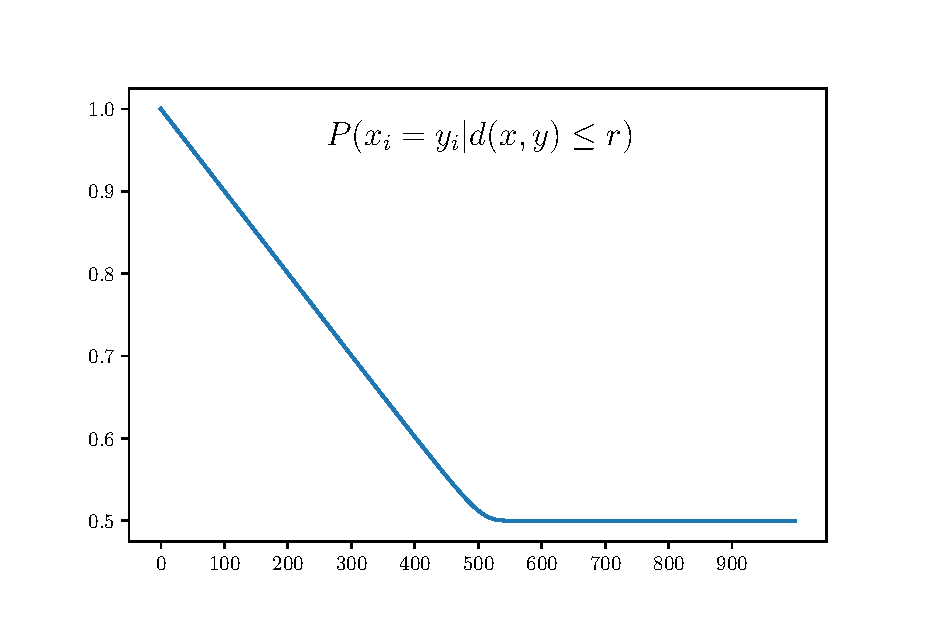
\includegraphics[width=0.5\textwidth]{./images02/autocorrelation/autocorrelation_n=1000_closeview=False.eps}

\caption{The threshold size $r$ of hard-locations bring about the autocorrelation of Theorem \ref{T1}. Consider, for instance, the extremes \{0, $n$\}.  Let us start with $n$ (in our case, $n=1000$ dimensions): given the information that $d(x,y)\le n$, the probability of a bitmatch in dimension $i$ is $1/2$; as $\forall x,y \in \{0, 1\}^N, d(x,y)\le n$. At the other extreme, consider that we have the information that $d(x,y)\le 0$: in this case $x=y$ and the probability of a bitmatch, in any dimension, is 1. The autocorrelation hence drops monotonically until convergence at $1/2$ as the distance grows. Numerically, our results converge to precisely $1/2$ only after $d(x,y)\ge 607$ for $n=1000$; $d(x,y)\ge 5332$ for $n=10000$, and $d(x,y)\ge 83$ for $n=100$. This will be seen in Lemma \ref{thm:sdm-access-radius}.
\label{fig:bitmatchbias}}
\end{figure}

\begin{lemma}
Let $r$ be the access radius given that $f$ percent of the hard locations are activated. Then, $\lim_{n \rightarrow \infty} r/n = 1/2$.
\label{thm:sdm-access-radius}
\end{lemma}
\begin{proof}

As the bits of the hard locations' addresses are randomly chosen, the distance between two hard locations follow a Binomial distribution with $n$ samples and probability 0.5, $B(n, 0.5)$. For $n$ sufficiently large, the Binomial distribution can be approximated by a Normal distribution, i.e., $B(n, 0.5) \rightarrow \mathcal{N}(\mu = n/2, \sigma^2 = n/4)$.

Let $\Phi(x)$ be the cdf of the standard normal distribution. Let $z = \frac{r - n/2}{\sqrt{n}/2}$. Thus, $P(d(x, y) \le r) = \Phi(z)$. As $f = P(d(x, y) \le r)$, then, $f = \Phi(z)$.

Calculating the inverse, $z = \Phi^{-1}(f)$. Then,

\begin{align}
z &= \Phi^{-1}(f) \\
\frac{r - n/2}{\sqrt{n}/2} &= \Phi^{-1}(f) \\
r &= \frac{n}{2} + \Phi^{-1}(f) \frac{\sqrt{n}}{2} \\
\frac{r}{n} &= \frac{1}{2} + \Phi^{-1}(f) \frac{1}{2 \sqrt{n}}
\end{align}

Therefore, $n \rightarrow \infty \Rightarrow r/n \rightarrow 1/2$.
\end{proof}

\begin{lemma}
Let $\Phi(x)$ be the cdf of the standard normal distribution. Then, $n \rightarrow \infty \Rightarrow P(x_i = y_i | d(x, y) \le r) = \frac{1}{2} \frac{\Phi(z_1)}{\Phi(z_2)}$, where $z_1 = \frac{2r - n + 1}{\sqrt{n-1}}$ and $z_2 = \frac{2r - n}{\sqrt{n}}$.
\label{thm:sdm-T1-n-large}
\end{lemma}
\begin{proof}

From the approximation of the Binomial distribution $B(a, 0.5)$ by the Normal distribution $\mathcal{N}(\mu = a/2, \sigma^2 = a/4)$, we conclude that, for $a$ sufficiently large, the cdf of the Binomial is approximately equal to the cdf of the Normal distribution. Thus,

$$
\frac{1}{2^a} \sum_{k=0}^{b} \binom{a}{k} = \Phi \left( \frac{b-a/2}{\sqrt{a}/2} \right) = \Phi \left( \frac{2b-a}{\sqrt{a}} \right)
$$

Thus,

$$
\sum_{k=0}^{b} \binom{a}{k} = 2^a \Phi \left( \frac{2b-a}{\sqrt{a}} \right)
$$

The result comes directly from applying the equation above in $P(x_i = y_i | d(x, y) \le r)$.

\end{proof}

\begin{theorem}
The autocorrelation vanishes when $n \rightarrow \infty$, i.e., $\lim_{n \rightarrow \infty} P(x_i = y_i | d(x, y) \le r) = 1/2$.
\label{thm:sdm-autocorrelation-convergence}
\end{theorem}
\begin{proof}

From Lemma \ref{thm:sdm-access-radius}, we know that $r = n/2$ for $n$ sufficiently large. Thus, replacing $r = n/2$ in Lemma \ref{thm:sdm-T1-n-large}, $P(x_i = y_i | d(x, y) \le r) = \frac{\Phi(z_1)}{2 \Phi(z_2)}$, where $z_1 = \frac{1}{\sqrt{n-1}}$ and $z_2 = 0$.

As $n \rightarrow \infty$, $z_1 \rightarrow 0$, and $P(x_i = y_i | d(x, y) \le r) = \frac{\Phi(0)}{2 \Phi(0)} = 1/2$. \qed

Another way to prove is to divide into two cases:

Suppose that $n$ is an even integer, then,

$$
\sum_{k=0}^{r} \binom{n}{k} = \sum_{k=0}^{n/2} \binom{n}{k} = \frac{1}{2} \sum_{k=0}^{n} \binom{n}{k} = \frac{2^n}{2} = 2^{n-1}
$$

And, also,

\begin{align*}
\sum_{k=0}^{r} \binom{n-1}{k} &= \sum_{k=0}^{n/2} \binom{n-1}{k} \\
    &= \frac{1}{2} \left[ \sum_{k=0}^{n-1} \binom{n-1}{k} - \binom{n-1}{n/2} \right] \\
    &= \frac{1}{2} \left[ 2^{n-1} - \binom{n-1}{n/2} \right] \\
    &= 2^{n-2} - \frac{1}{2} \binom{n-1}{n/2}
\end{align*}

Finally,

\begin{align}
P(x_i = y_i | d(x, y) \le r) &= \frac{\sum_{k=0}^{r} \binom{n-1}{k}}{\sum_{k=0}^{r} \binom{n}{k}} \\
    &= \frac{2^{n-2} - \frac{1}{2} \binom{n-1}{n/2}}{2^{n-1}} \\
    &= \frac{2^{n-2}}{2^{n-1}} - \frac{1}{2^n} \binom{n-1}{n/2} \\
    &= \frac{1}{2} - \frac{1}{2^n} \binom{n-1}{n/2}
\end{align}

Stirling's approximation yields that, for $n$ sufficiently large, $\binom{n}{n/2} \sim \frac{2^n}{\sqrt{\pi n/2}}$. Thus, $\frac{1}{2^n} \binom{n}{n/2} \sim \frac{\sqrt{2}}{\sqrt{\pi n}}$, which yields $\lim_{n \rightarrow \infty} \frac{1}{2^n} \binom{n}{n/2} = 0$. Finally, as $\binom{n-1}{n/2} \le \binom{n}{n/2}$, by the squeeze theorem, $\lim_{n \rightarrow \infty} \frac{1}{2^n} \binom{n-1}{n/2} = 0$, which closes the proof for $n$ even.

When $n$ is an odd integer, the steps of the proof are similar. Therefore, the proof is complete.

\end{proof}

In Figure \ref{fig:sdm-10kbits-figure-7-3}, with $n=10,000$ and $r=4,845$, we can notice that the autocorrelation has reduced significantly as predicted by Theorem \ref{thm:sdm-autocorrelation-convergence}. In fact, in this case, using Lemma \ref{thm:sdm-T1-n-large}, $P(x_i = y_i | d(x, y) \le r) = 0.516876$.

\begin{figure}[!htb]
  \centering
  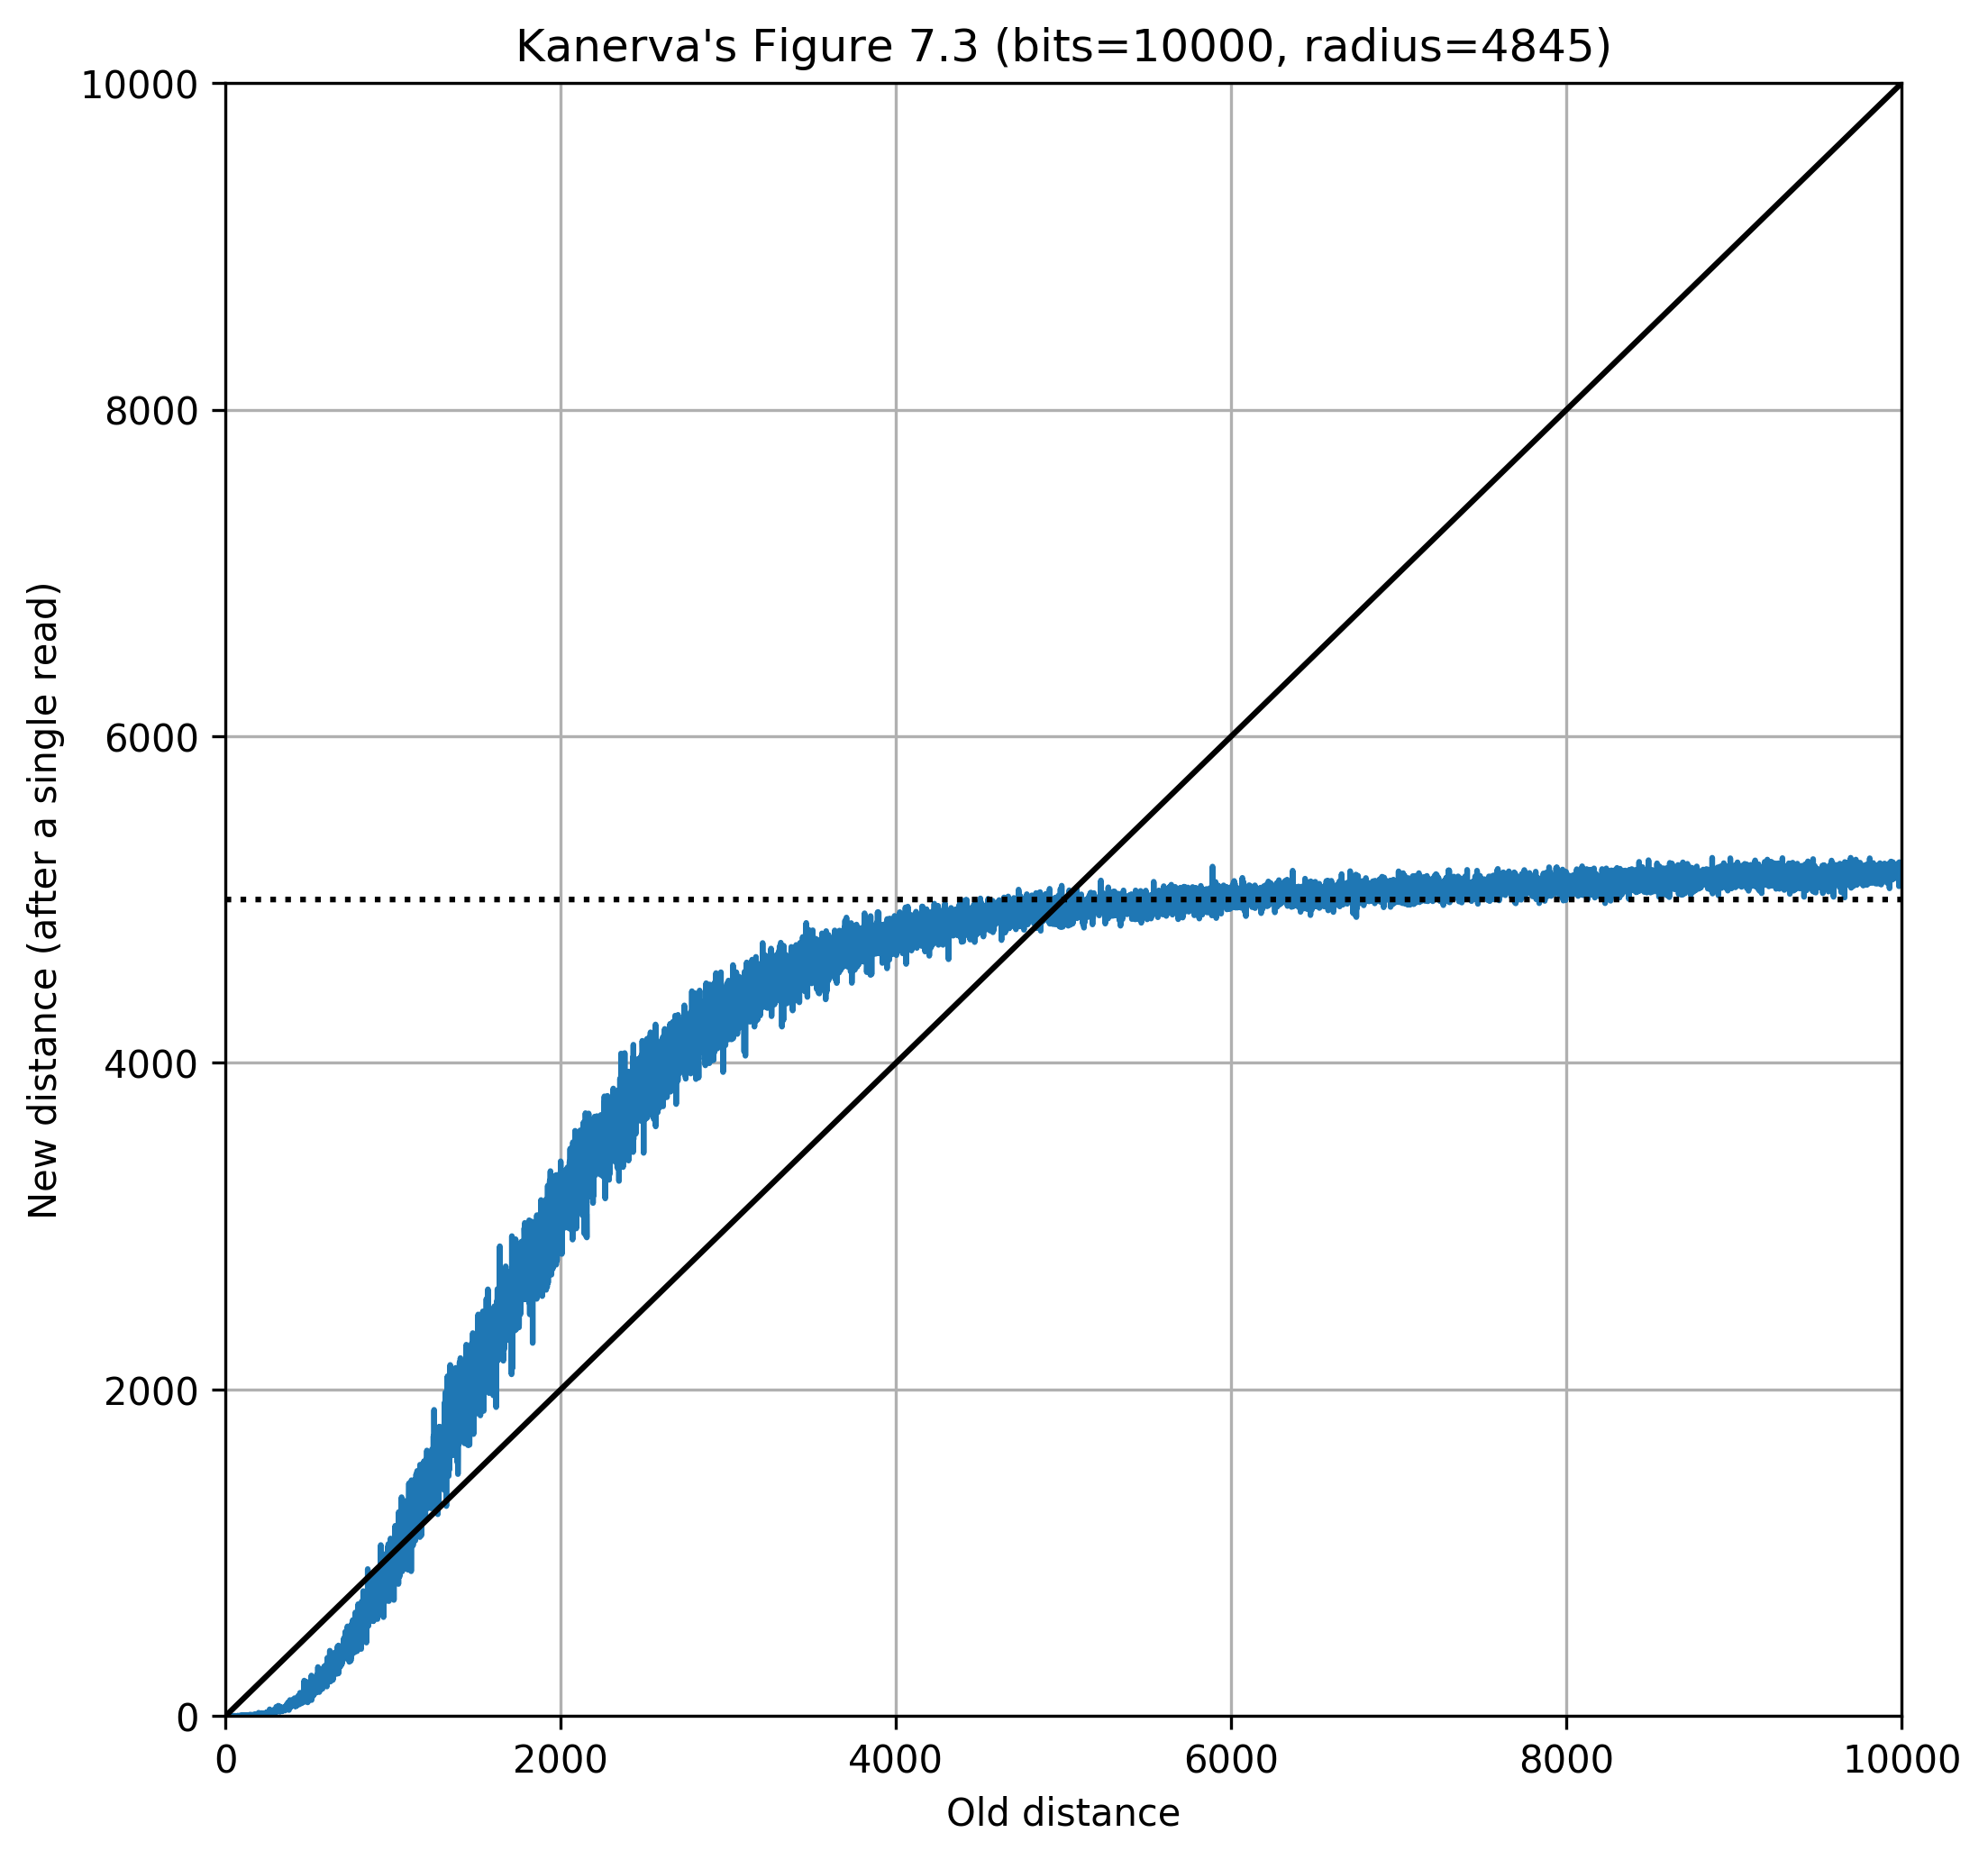
\includegraphics[width=0.5\textwidth]{./images02/sdm-10000bits-10000w-table-7-2.png}

  \caption{The same setup as in Figure \ref{fig:sdm-10000w-table-7-2}, but for $n=10,000$. It shows that the interference has almost gone away when $n$ is sufficiently large.}
  \label{fig:sdm-10kbits-figure-7-3}
\end{figure}

So far we have looked only at a single pair of bitstrings, the probability of a single bitmatch between bitstrings within the access radius distance.  Now let us consider the number of activated hard locations exhibiting this bitmatch.

Let $h$ be the number of activated hard locations. As the probability of activating a specific hard location is a constant $h \sim \text{Binomial}(H, p_1)$. Thus, $\mathbf{E}[h] = \mu_h = Hp_1$ and $\mathbf{V}[h] = \sigma^2_h = Hp_1(1-p_1)$, where $p_1 = 2^{-n} \sum_{k=0}^{r} \binom{n}{k}$.

Let $Z$ be the number of activated hard locations with the same bit as the reading address. Then, $Z = \sum_{i=1}^{h} X_i$, where $X_i \sim \text{Bernoulli}(p)$, where $p = P(x_i = y_i | d(x, y) \le r)$.

\begin{theorem}
Given a reading address $x$ and a dimension $i$, the number of activated hard-locations with bitmatches at $i$ follows a normal distribution with $\mathbf{E}[Z] = \mu_Z = p \mu_h$ and $\mathbf{V}[Z] = \sigma_Z^2 = p(1-p) \mu_h + p^2 \sigma^2_h$.
\label{T2}
\end{theorem}

\begin{proof}
By the central limit theorem, $Z$ is normally distributed.

Applying the law of total averages and the law of total variance, $\mathbf{E}[Z] = \mathbf{E}[\mathbf{E}[Z | h]] = \mathbf{E}[ph] = p \mathbf{E}[h] = ph$, and $\mathbf{V}[Z] = \mathbf{E}[\mathbf{V}[Z|h]] + \mathbf{V}[\mathbf{E}[Z|h]] = \mathbf{E}[hp(1-p)] + \mathbf{V}[ph] = p(1-p) \mathbf{E}[h] + p^2 \mathbf{V}[h] = hp(1-p) + p^2 H p_1 (1-p_1)$.

Applying the law of total variance, $\mathbf{V}[Z] = \mathbf{E}[\mathbf{V}[Z|h]] + \mathbf{V}[\mathbf{E}[Z|h]] = \mathbf{E}[hp(1-p)] + \mathbf{V}[ph] = p(1-p) \mathbf{E}[h] + p^2 \mathbf{V}[h] = p(1-p)\mu_h + p^2 \sigma^2_h$.
\end{proof}
As, in our case, $P(973 < h < 1170) = 0.997$, by the central limit theorem, $Z$ may be approximated by a normal distribution.

See Figure \ref{fig:sdm-same-bit-histogram} for a comparison between the theoretical model and a simulation.

\begin{figure}[h!]
  \centering
  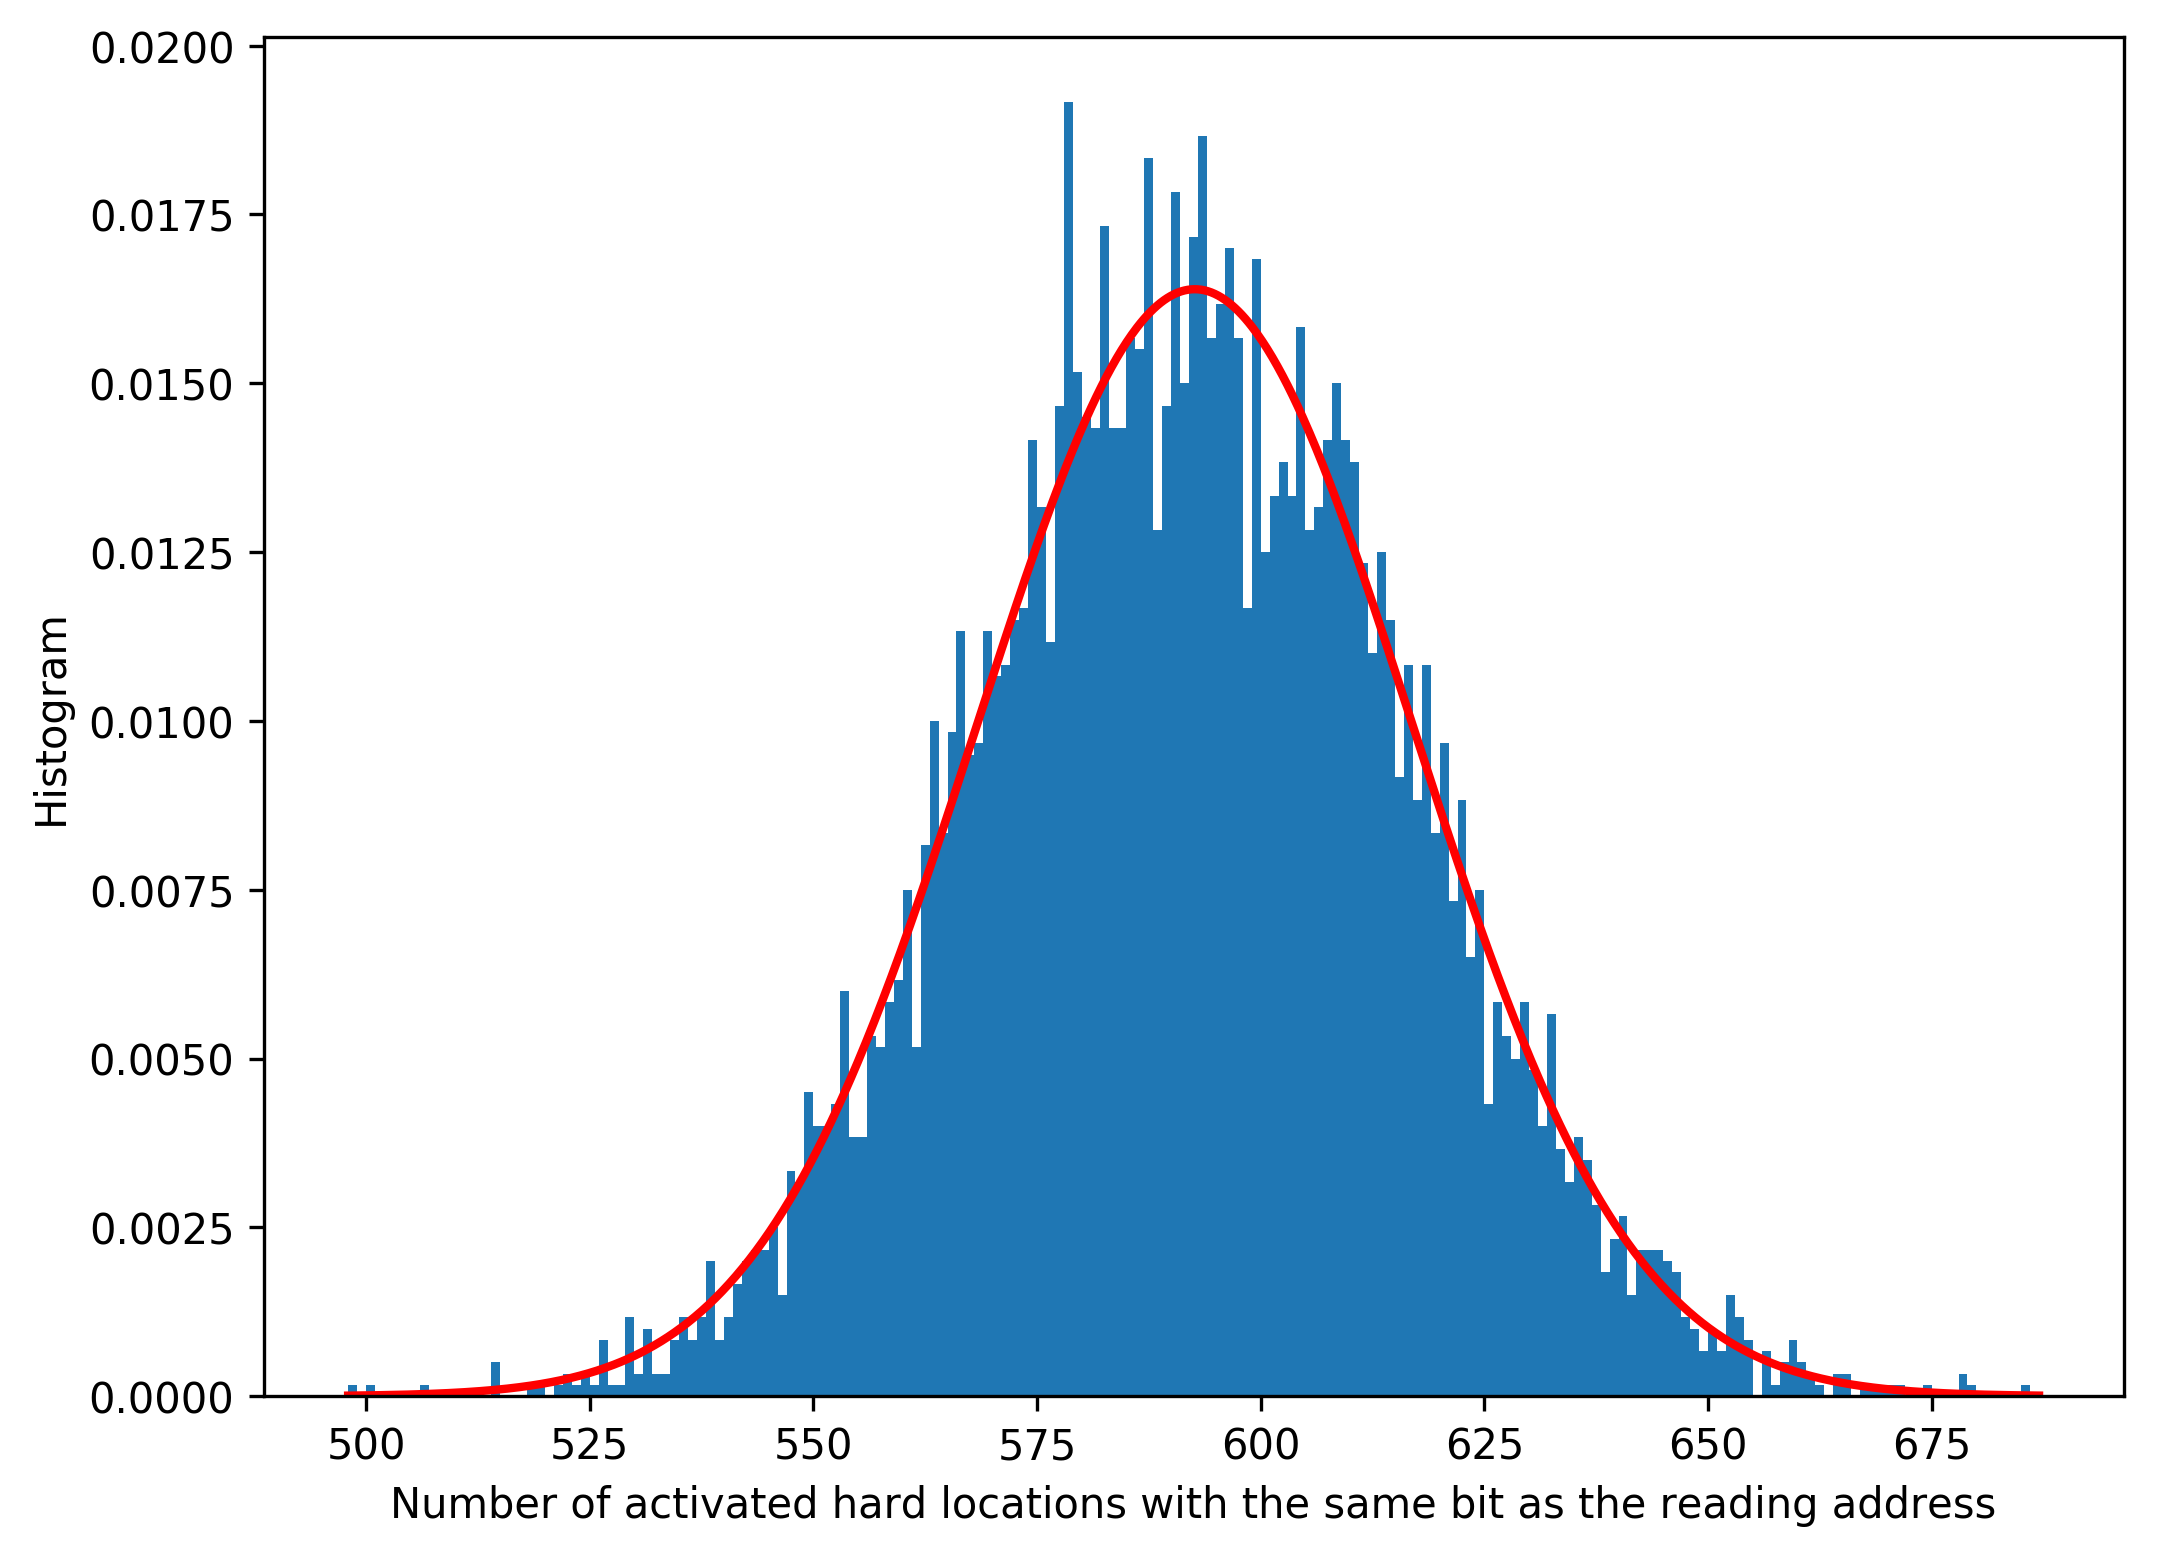
\includegraphics[width=0.5\textwidth]{./images02/autocorrelation/same-bit-histogram.png}

  \caption{Given an address $x$ and a dimension $i$, how many hard locations with bitmatches in $i$ are activated by reading at $x$?  The histogram was obtained through numerical simulation. The red curve is the theoretical normal distribution found in Theorem \ref{T2}.}
  \label{fig:sdm-same-bit-histogram}
\end{figure}

\section{Counter bias}

The previous theorems show that there is bias in the counters. In this section we show that there is a small counter bias, as a function of the bitmatch in dimension $i$. If the Hard location's address bit is set to 1, the mean will be above zero.  And the mean will be below zero if the address bit is set to 0.

Let us analyze the $i$th counter of a hard location.  Let $s$ be the number of bitstrings written into memory (in our case, $s=10,000$) and $\text{addr}_i$ be the $i$th bit of the hard location's address.

Let $\theta$ be the average number of bitstrings written in each hard location. As there are $s$ bitstrings written into the memory, and the probability of activating a specific hard location is constant, $\theta \sim \text{Binomial}(s, p_1)$. Thus, $\mathbf{E}[\theta] = \mu_\theta = s p_1$ and $\mathbf{V}[\theta] = \sigma^2_\theta = s p_1 (1 - p_1)$.

Let us introduce another random variable.  Let $Y_i$ be the number of bitmatches in the $i$th dimension of a hard location's address after $s$ written bitstrings. Then, $Y_i = \sum_{k=1}^{\theta} X_k$.

\begin{theorem}
Given the number of written bitstrings $s$, $\mathbf{E}[Y_i] = \mu_Y = p \mu_\theta$ and $\mathbf{V}[Y_i] = \sigma^2_Y = p(1-p) \mu_\theta + p^2 \sigma^2_\theta$.
\end{theorem}
\begin{proof}
Applying the law of total expectation, $\mathbf{E}[Y] = \mathbf{E}[\mathbf{E}[Y|\theta]] = \mathbf{E}[p \theta] = p \mathbf{E}[\theta] = p \mu_\theta$.

Applying the law of total variance, \\
$\mathbf{V}[Y] = \mathbf{E}[\mathbf{V}[Y|\theta]] + \mathbf{V}[\mathbf{E}[Y|\theta]] = \mathbf{E}[\theta p (1-p)] + \mathbf{V}[p \theta] = p(1-p) \mathbf{E}[\theta] + p^2 \mathbf{V}[\theta] = p(1-p) \mu_\theta + p^2 \sigma^2_\theta$.
\end{proof}

During a write operation, the counters are incremented for every bit 1 and decremented for every bit 0. So, after $s$ writes, there will be $\theta$ bitstrings written in each hard location with $Y_i$ bitmatches and $\theta - Y_i$ non-bitmatches. Thus, $[\text{cnt}_i | \text{addr}_i = 1] = (Y_i) - (\theta - Y_i) = 2Y_i - \theta$ and $[\text{cnt}_i | \text{addr}_i = 0] = \theta - 2Y_i$.

\begin{theorem}
$\mathbf{E}[\text{cnt}_i | \text{addr}_i = 1] = \mu_{\text{cnt}} = (2p-1) \mu_\theta$ and $\mathbf{V}[\text{cnt}_i | \text{addr}_i = 1] = \sigma^2_\text{cnt} = 4p(1-p) \mu_\theta + (2p-1)^2 \sigma^2_\theta$.
\end{theorem}

\begin{proof}

$\mathbf{E}[\text{cnt}_i | \text{addr}_i = 1] = \mathbf{E}[2Y_i - \theta] = \mathbf{E}[2Y_i] - \mathbf{E}[\theta] = 2 \mathbf{E}[Y_i] - \mu_\theta = 2 p \mu_\theta - \mu_\theta = (2p-1) \mu_\theta$.

Applying the law of total variance, $\mathbf{V}[\text{cnt}_i | \text{addr}_i = 1] = \mathbf{V}[2Y_i - \theta] = \mathbf{E}[\mathbf{V}[2Y_i - \theta | \theta]] + \mathbf{V}[\mathbf{E}[2Y_i - \theta | \theta]]$.

Let us solve each part independently. Thus,

$\mathbf{V}[2Y_i - \theta | \theta] = \mathbf{V}[2Y_i | \theta] = 4 \mathbf{V}[Y_i | \theta] = 4 \mathbf{V}[\sum_{k=1}^\theta X_k] = 4 \theta p (1-p)$.

$\mathbf{E}[\mathbf{V}[2Y_i - \theta | \theta]] = \mathbf{E}[4 \theta p (1-p)] = 4p(1-p) \mathbf{E}[\theta] = 4p(1-p) \mu_\theta$.

Finally,

$\mathbf{E}[2Y_i - \theta | \theta] = 2 \mathbf{E}[Y_i | \theta] - \mathbf{E}[\theta | \theta] = 2p \theta - \theta = (2p-1) \theta$.

$\mathbf{V}[\mathbf{E}[2Y_i - \theta | \theta]] = \mathbf{V}[(2p-1) \theta] = (2p-1)^2 \mathbf{V}[\theta] = (2p-1)^2 \sigma^2_\theta$.
\end{proof}

\begin{theorem}
$\mathbf{E}[\text{cnt}_i | \text{addr}_i = 0] = - \mu_{\text{cnt}}$ and $\mathbf{V}[\text{cnt}_i | \text{addr}_i = 1] = \sigma^2_\text{cnt}$.
\end{theorem}
\begin{proof}
Notice that $[\text{cnt}_i | \text{addr}_i = 0] = -[\text{cnt}_i | \text{addr}_i = 1]$. Thus, $\mathbf{E}[\text{cnt}_i | \text{addr}_i = 0] = -\mathbf{E}[\text{cnt}_i | \text{addr}_i = 1]$ and $\mathbf{V}[\text{cnt}_i | \text{addr}_i = 0] = \mathbf{V}[\text{cnt}_i | \text{addr}_i = 1]$.
\end{proof}

In summary, what we learn is that

\begin{align}
\left[ \text{cnt}_i | \text{addr}_i=1 \right] &\sim \mathcal{N}(\mu_\text{cnt}, \sigma^2_\text{cnt})\label{cntaddr1} \\
\left[ \text{cnt}_i | \text{addr}_i=0 \right] &\sim \mathcal{N}(-\mu_\text{cnt}, \sigma^2_\text{cnt})\label{cntaddr0}
\end{align}

In our case, $p=0.5529$, $s=10,000$, and $H=1,000,000$, so $[\text{cnt}_i | \text{addr}_i=1] \sim \mathcal{N}(\mu=1.1341, \sigma^2 = 10.7184)$. For ``random at x'', $p=0.5$, so $\mu = 0$ and $\sigma^2 = 10.7185$. The slight bias above or below 0 can be seen in Figure \ref{fig:sdm-corr-counters}.

\begin{figure}[h!]
  \centering
  \subfloat[$\text{addr}_i=1$]{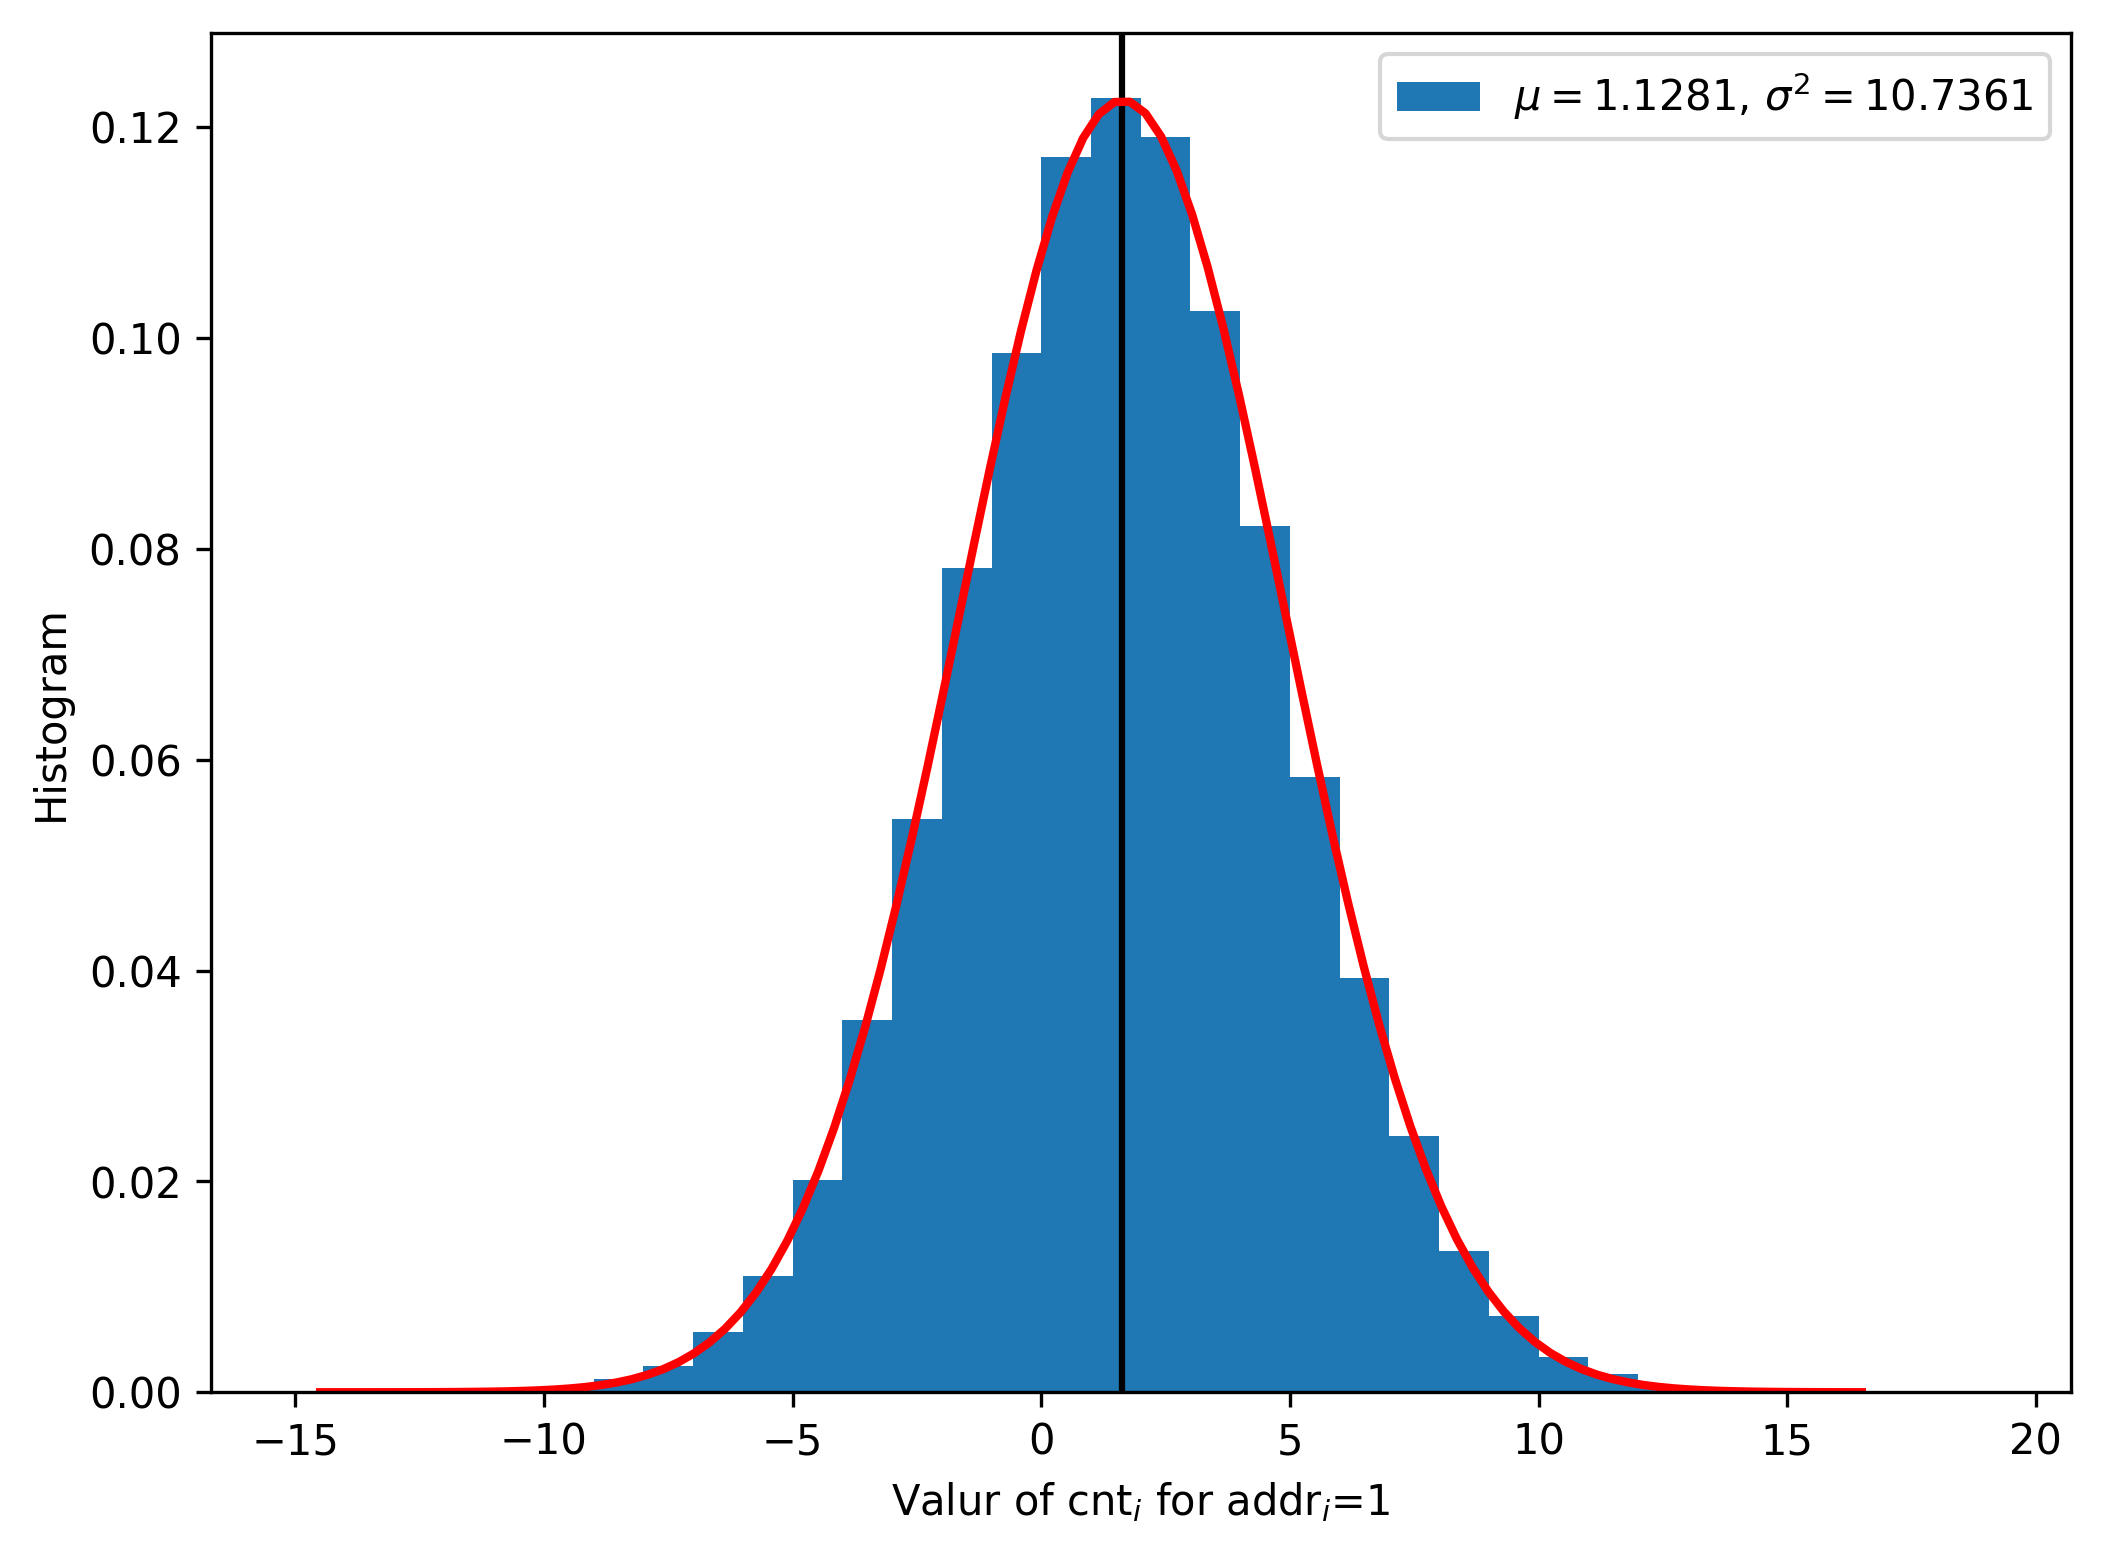
\includegraphics[width=0.5\textwidth]{./images02/autocorrelation/x_at_x_addr1.png}}

  \subfloat[$\text{addr}_i=0$]{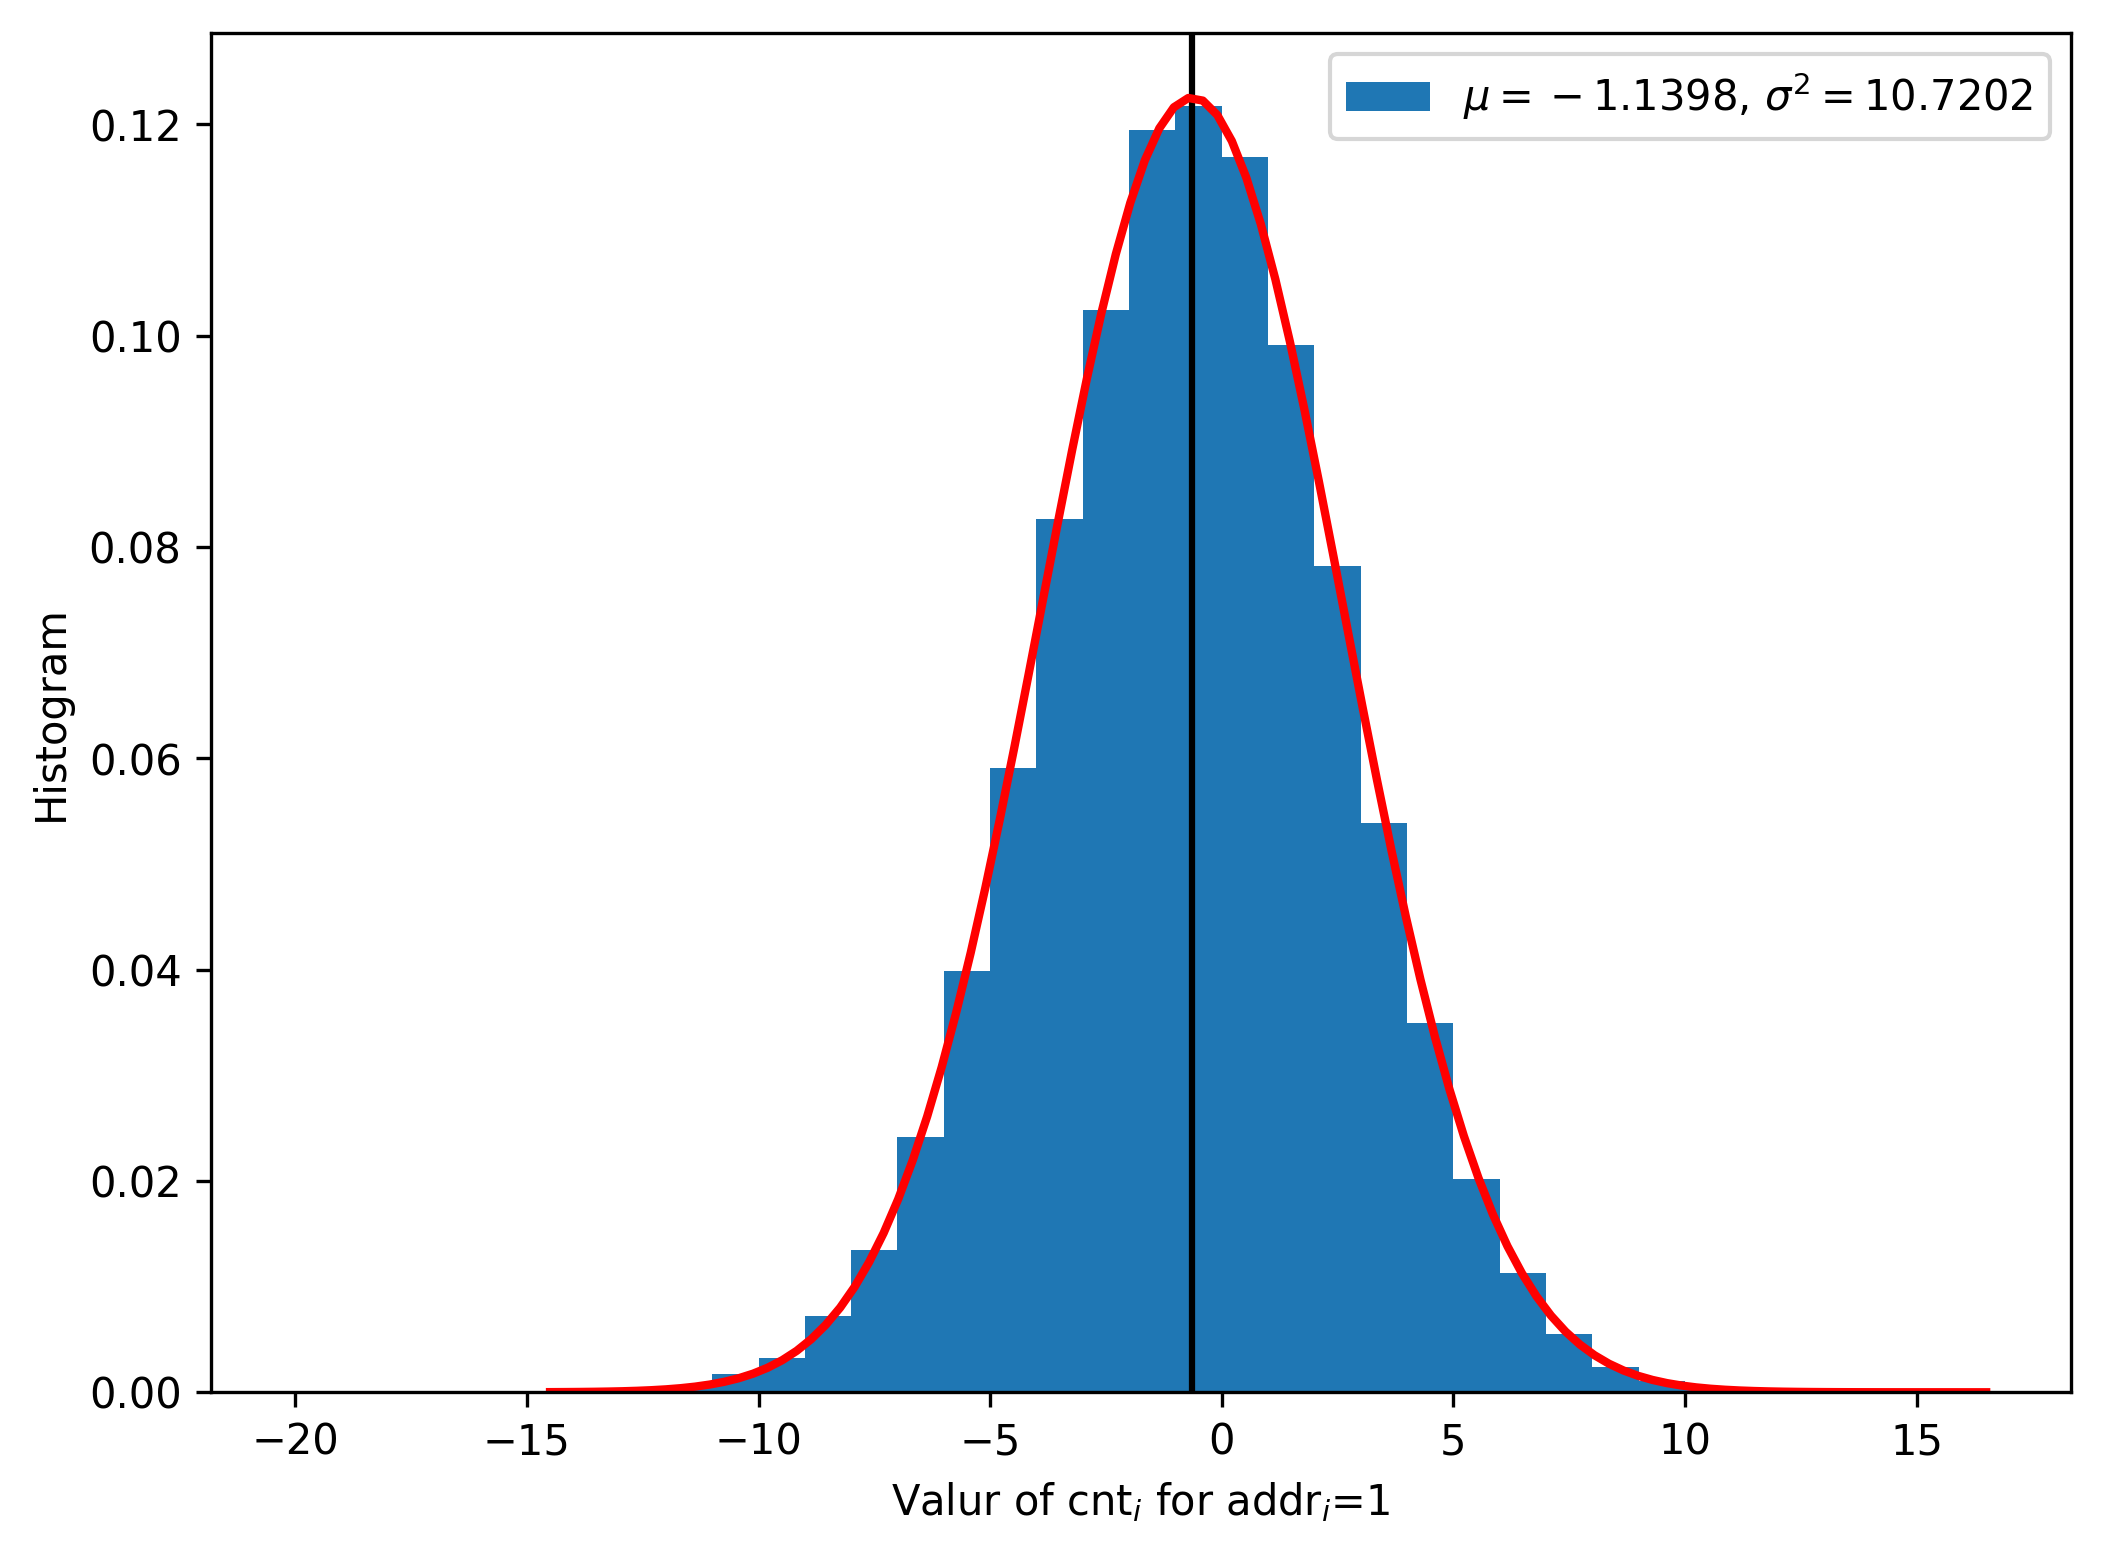
\includegraphics[width=0.5\textwidth]{./images02/autocorrelation/x_at_x_addr0.png}}

  \caption{The value of the counters after $s=10,000$ writes shows the autocorrelation in the counters in autoassociative memories (``x at x''). The histogram was obtained through simulation. The red curve is the theoretical normal distribution found in equations (\ref{cntaddr1}) and (\ref{cntaddr0}).}
  \label{fig:sdm-corr-counters}
\end{figure}


Finally,

\begin{align}
P(\text{cnt}_i \ge 0 | \text{addr}_i = 1) = P(\text{cnt}_i \le 0 | \text{addr}_i = 0) \\
 = 1 - \mathcal{N}.\text{cdf}(0)
\end{align}

For ``random written at x'', $p=0.5$ implies $\mu_\text{cnt} = 0$, which implies $P(\text{cnt}_i \ge 0 | \text{addr}_i = 1) = P(\text{cnt}_i \le 0 | \text{addr}_i = 0) = 0.5$, independently of the parameters because they will only affect the variance and the normal distribution is symmetrical around the average.

However, for ``x written at x'', $p=0.5529$ and the probabilities depend on $s$. For $s=10,000$, they are equal to 0.6354. For $s=20,000$, they are equal to 0.6867. For $s=30,000$, they are equal to 0.7232. The more random bitstrings are written into the memory, the more the hard locations point to themselves.

Let $D$ be the number of counters aligned with $\text{addr}_i$. The standard deviation was calculated using the fact that $[D|\theta] \sim \text{Binomial}(1000, q=P(\text{cnt}_i > 0 | \text{addr}_i=1, \theta))$.

Applying the law of total variance, $\mathbf{V}[D] = \mathbf{E}[\mathbf{V}[D|\theta]] + \mathbf{V}[\mathbf{E}[D|\theta]] = \mathbf{E}[1000 q (1-q)] + \mathbf{V}[1000 q] = 1000 \mathbf{E}[q-q^2] + 1000^2 \mathbf{V}[q] = 1000 \mathbf{E}[q](1-\mathbf{E}[q]) + 1000(1000-1)\mathbf{V}[q]$, where $\mathbf{E}[q] = \sum_\theta P(\text{cnt}_i > 0 | \text{addr}_i=1, \theta) P(\theta)$ and $\mathbf{E}[q^2] = \sum_\theta [P(\text{cnt}_i > 0 | \text{addr}_i=1, \theta)]^2 P(\theta)$.

Doing the math, $\mathbf{E}[q] = 0.402922$ and $\mathbf{E}[q^2] = 0.634433$. Thus, $\mathbf{V}[q] = \mathbf{E}[q^2] - (\mathbf{E}[q])^2 = 0.0004166$. Hence, $\mathbf{V}[D] = 648.2041$. See Figure \ref{fig:sdm-corr-prob} and notice that I still have to figure out why the mean is correct, but the standard deviation is not.

\begin{figure}[h!]
  \centering
  \subfloat[``random at x'']{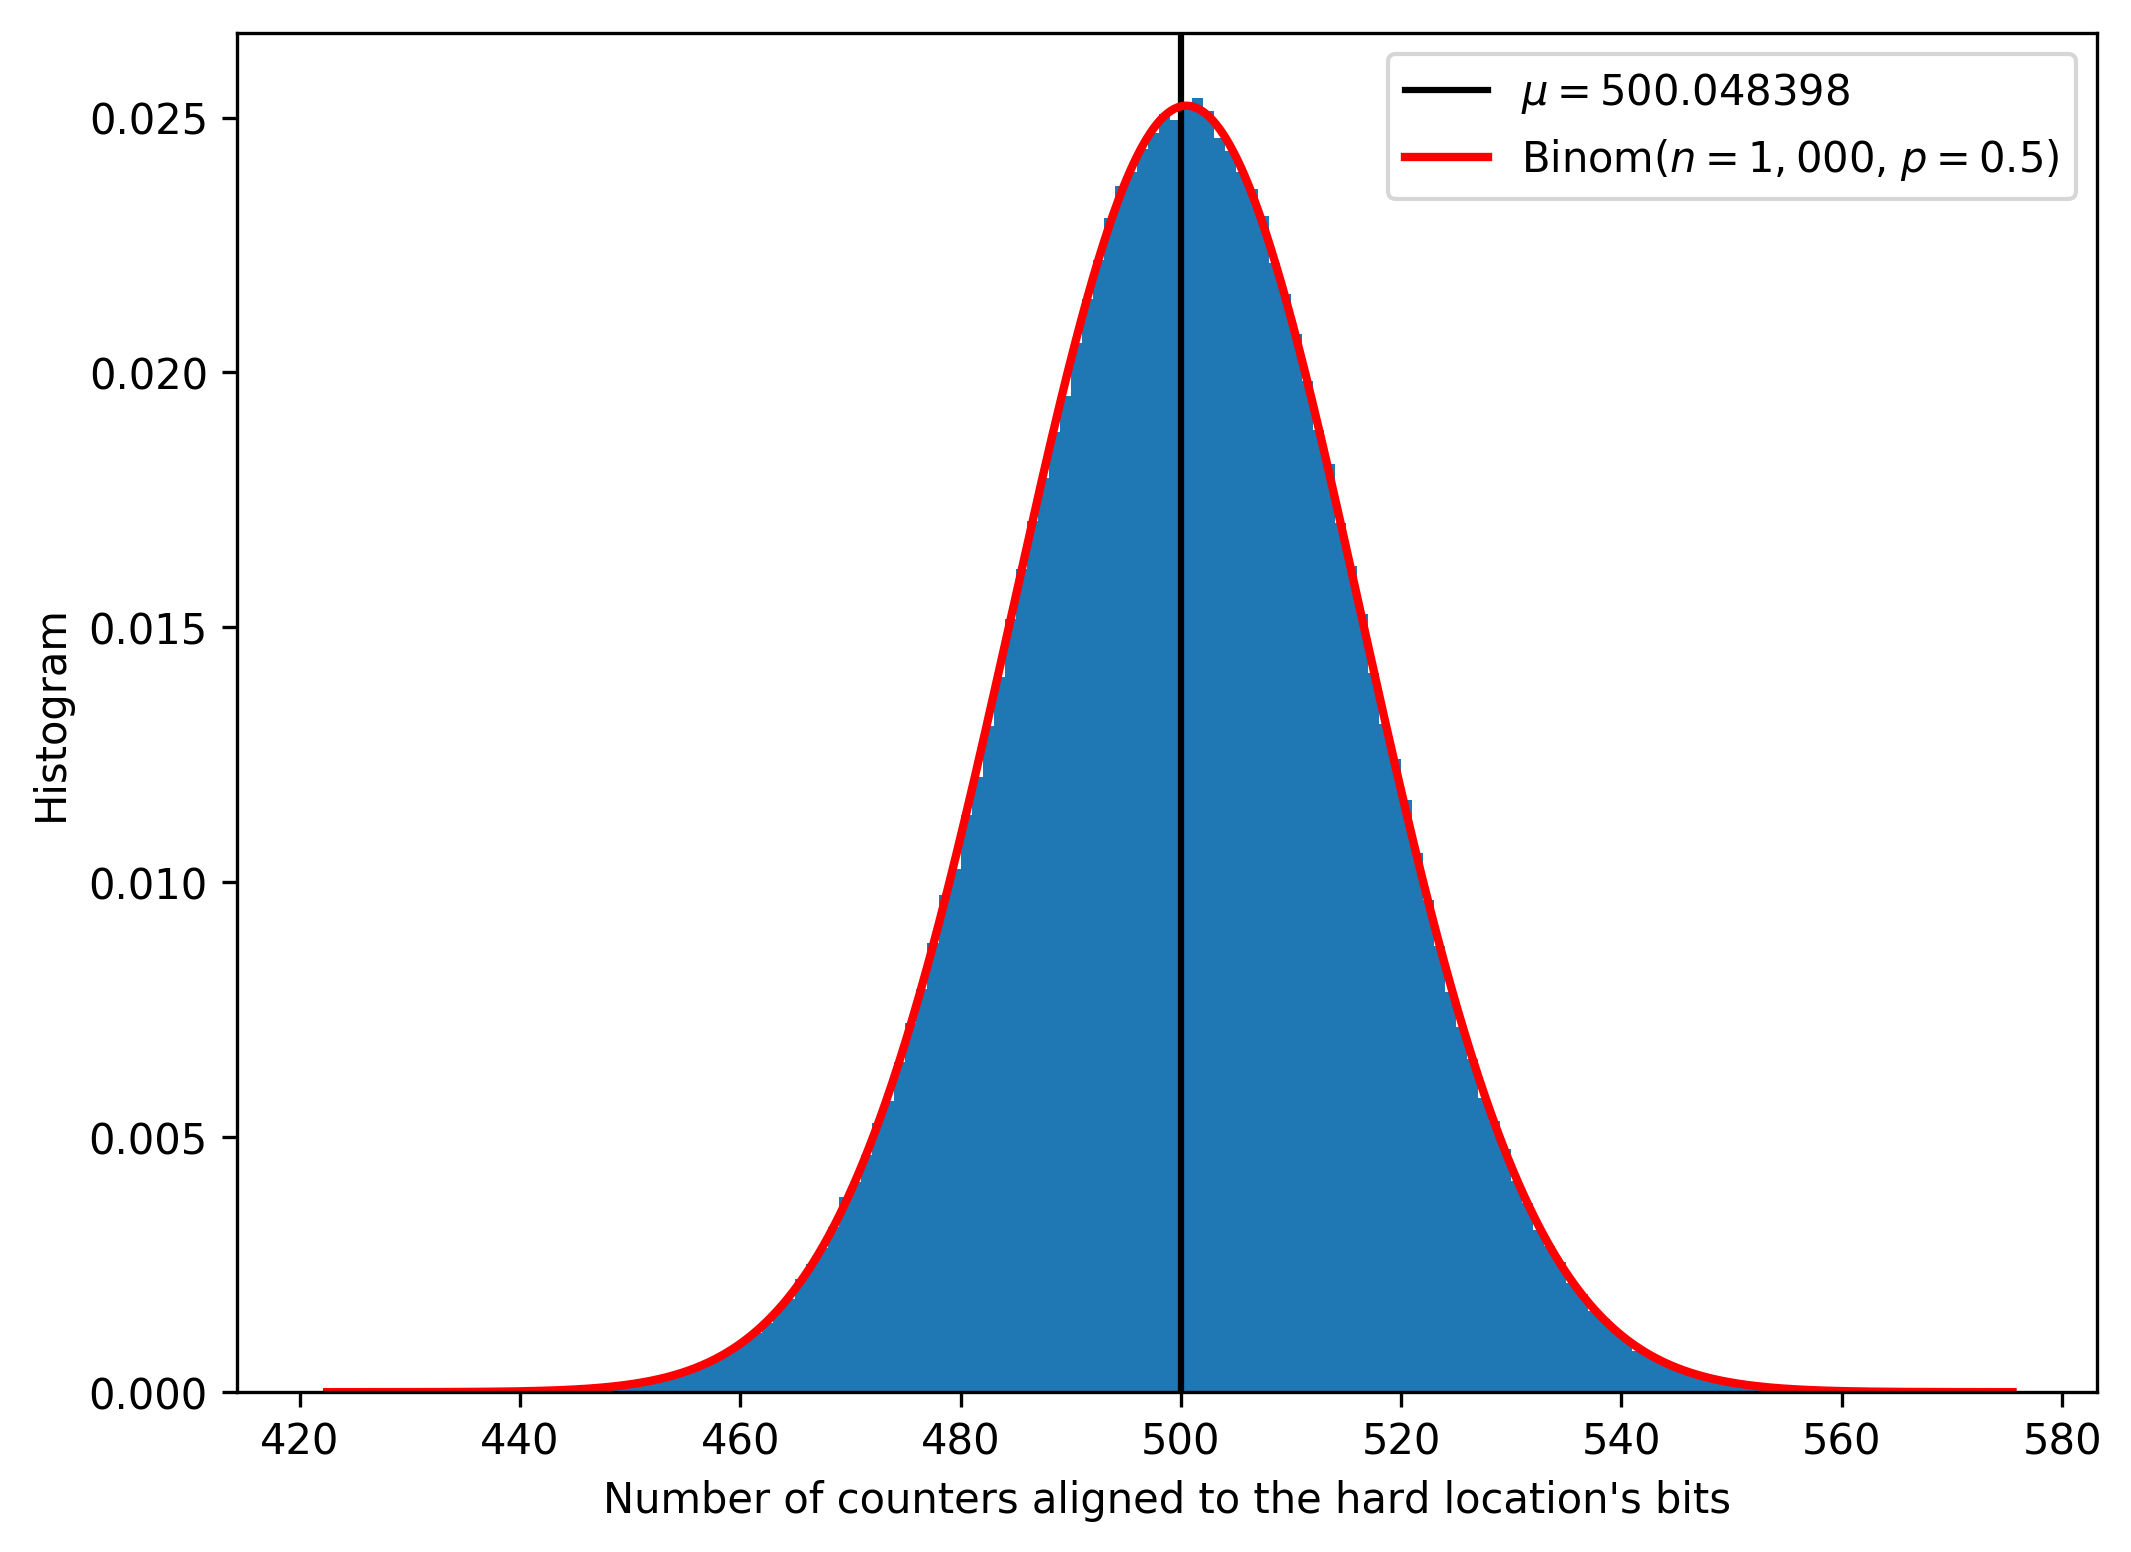
\includegraphics[width=0.5\textwidth]{./images02/autocorrelation/random_at_x_counters.png}}

  \subfloat[``x at x'']{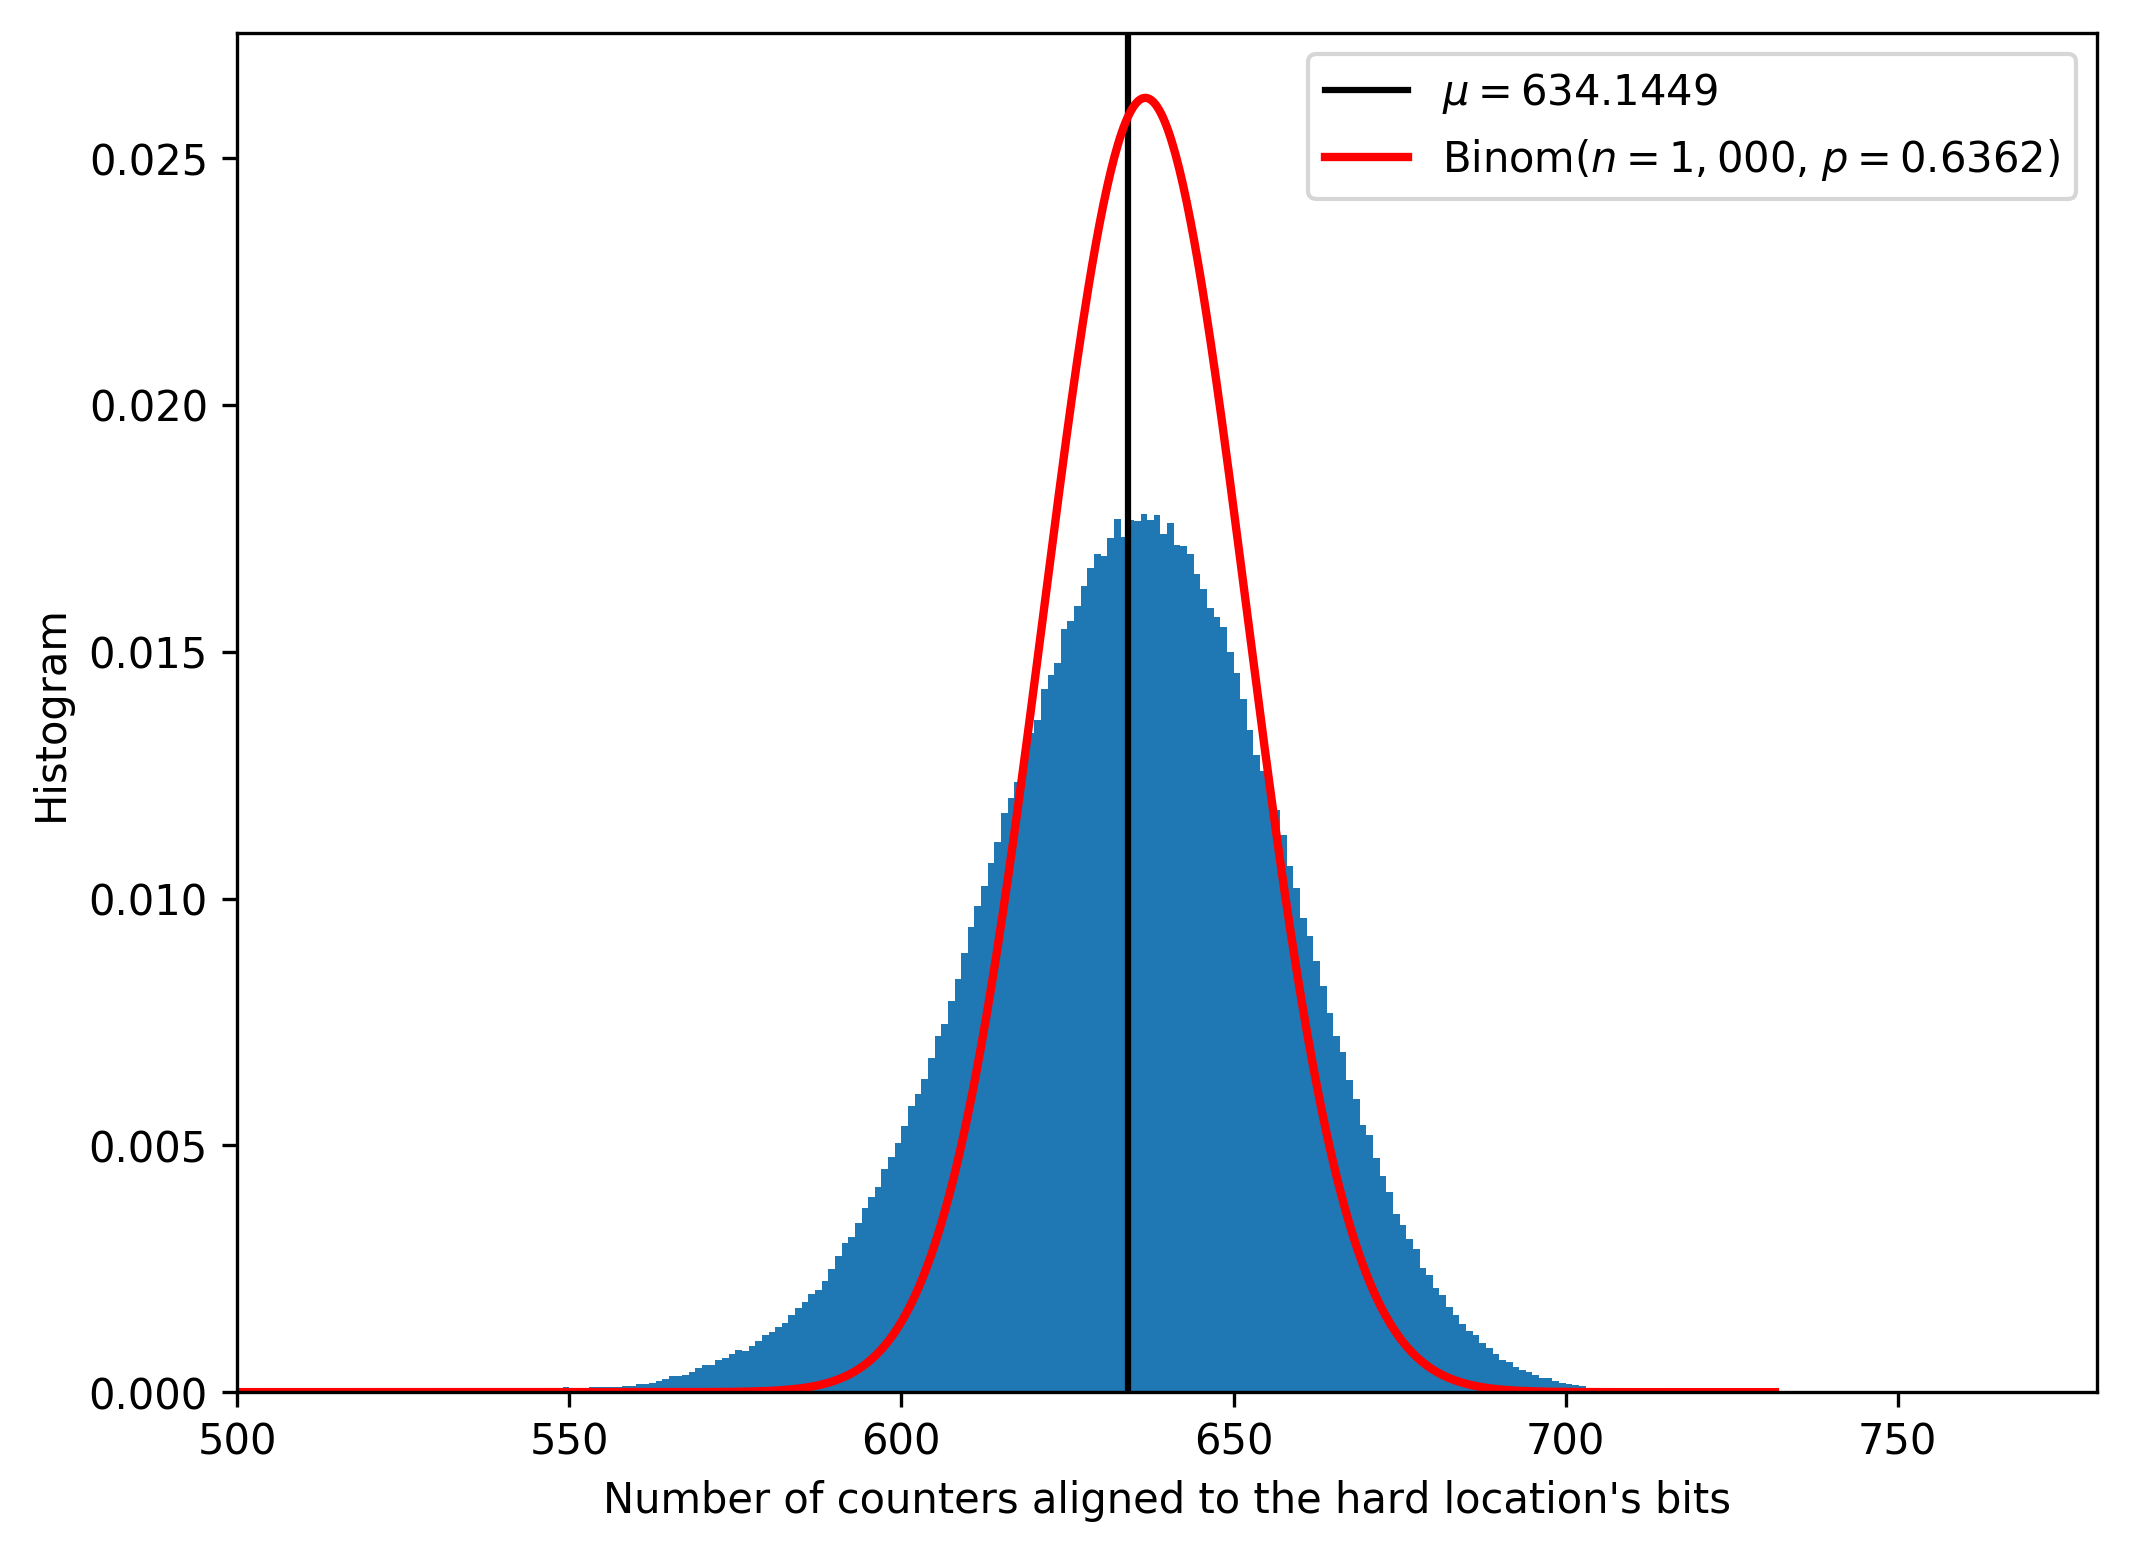
\includegraphics[width=0.5\textwidth]{./images02/autocorrelation/x_at_x_counters.png}}

  \caption{Autocorrelation in the counters in autoassociative memories (``x written at x''). The histogram was obtained through simulation. The red curve is the theoretical distribution.}
  \label{fig:sdm-corr-prob}
\end{figure}



\section{Read bias}

Now that we know the distribution of $\text{cnt}_i | \text{addr}_i$, we may go to the read operation. During the read operation, on average, $h$ hard locations are activated and their counters are summed up. So, for the $i$th bit,

\begin{align}
\text{acc}_i = \sum_{k=1}^{h} \text{cnt}_k
\end{align}

Let $\eta$ be the reading address and $\eta_i$ the $i$th bit of it. Then, let's split the $h$ activated hard locations into two groups: (i) the ones with the same bit as $\eta_i$ with $Z$ hard locations, and (ii) the ones with the opposite bit as $\eta_i$ with $h-Z$ hard locations.

\begin{align}
\left[ \text{acc}_i|\eta_i \right] &= \sum_{k=1}^{Z} \left[ \text{cnt}_k | \text{addr}_k=\eta_i \right] + \sum_{k=1}^{h-Z} \left[ \text{cnt}_k | \text{addr}_k \ne \eta_i \right]
\end{align}

Each sum is a sum of normally distributed random variables, so

\begin{align}
\begin{split}
\sum_{k=1}^{Z} \left[ \text{cnt}_k | \text{addr}_k=\eta_1 \right] &\sim \\
& \mathcal{N}(\mu = \mu_\text{cnt} \mu_Z, \sigma^2 = \sigma_\text{cnt}^2 \mu_Z + \mu_\text{cnt}^2 \sigma^2_Z) \label{eqn:sdm-eta1-addr1}
\end{split}
\end{align}
, and, respectively:

\begin{align}
\begin{split}
& \sum_{k=1}^{h-Z} \left[ \text{cnt}_k | \text{addr}_k \ne \eta_1 \right] \sim \\
& \mathcal{N}(\mu = -\mu_\text{cnt} (1-p) \mu_h, \sigma^2 = \sigma^2_\text{cnt} (1-p) \mu_h + \mu_\text{cnt}^2 \sigma^2_{h-Z}) \label{eqn:sdm-eta1-addr0}
\end{split}
\end{align}

In our case, $\sum_{k=1}^{Z} \left[ \text{cnt}_k | \text{addr}_k=1 \right] \sim \mathcal{N}(\mu=672.12, \sigma^2=7113.87)$, and $\sum_{k=1}^{Z} \left[ \text{cnt}_k | \text{addr}_k=1 \right] \sim \mathcal{N}(\mu=-543.49, \sigma^2=5752.54)$. See Figure \ref{fig:sdm-read-sums} --- we can notice that the average is correct but the variance is too small.

\begin{figure}[h!]
  \centering
  \subfloat[Equation \ref{eqn:sdm-eta1-addr1}  ($\text{addr}_k=1)$]{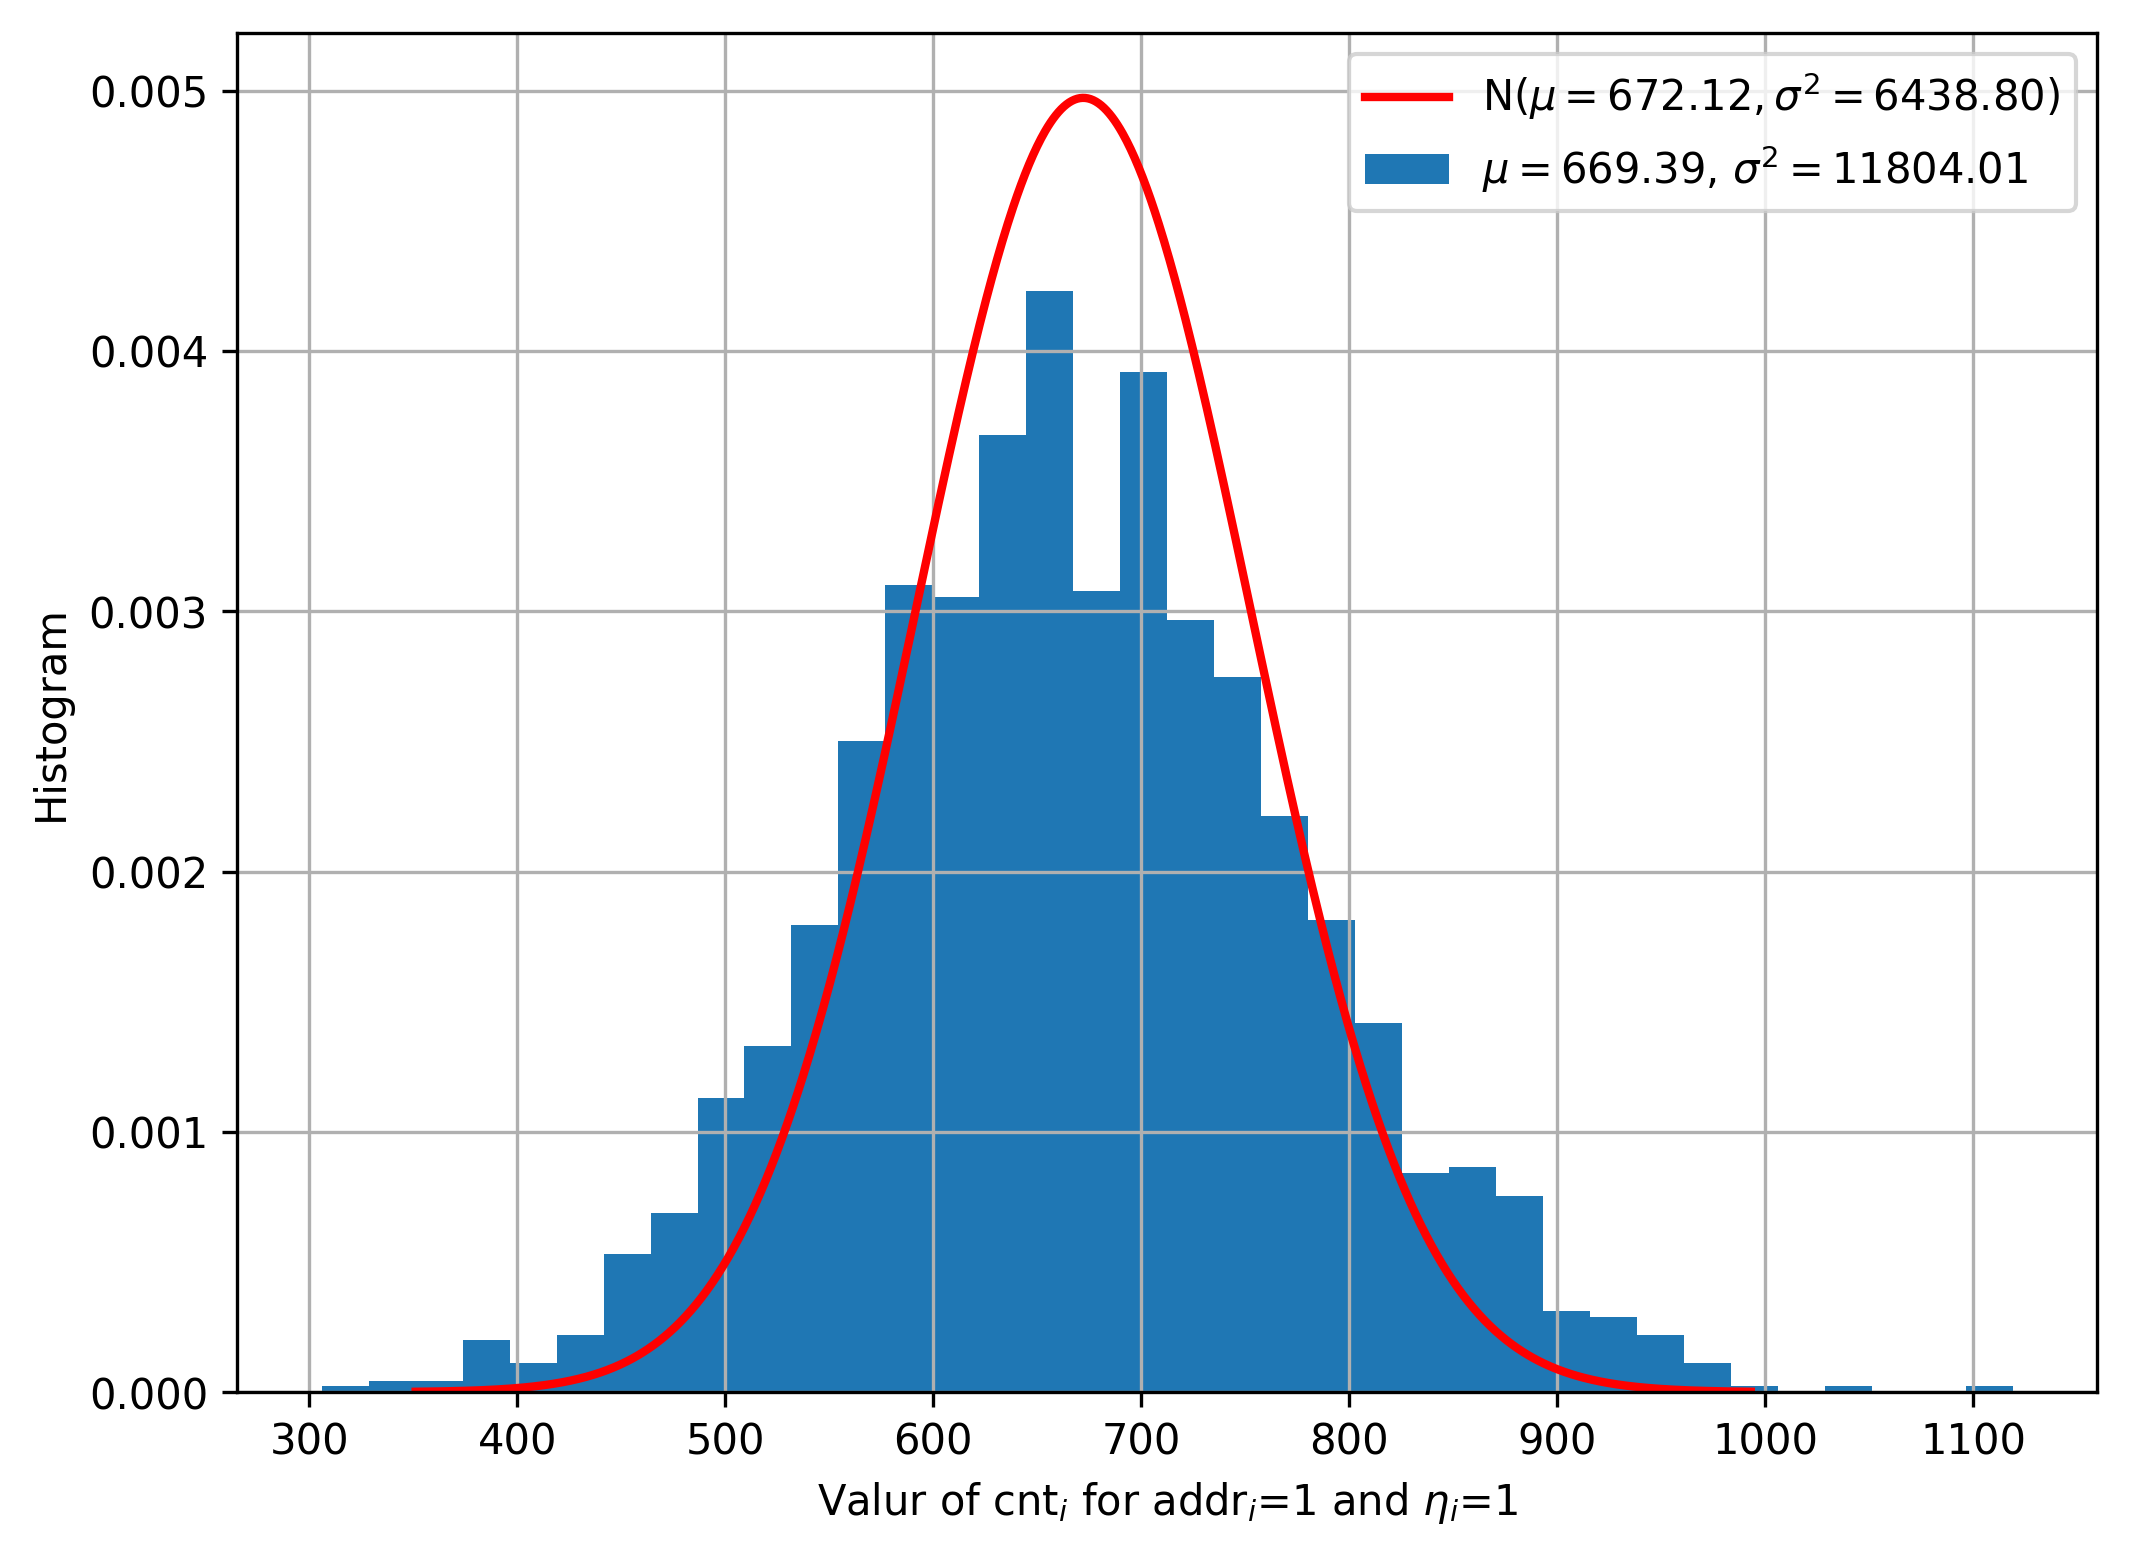
\includegraphics[width=0.5\textwidth]{./images02/autocorrelation/read-counters-eta1_addr1.png}}

  \subfloat[Equation \ref{eqn:sdm-eta1-addr0} ($\text{addr}_k=0$)]{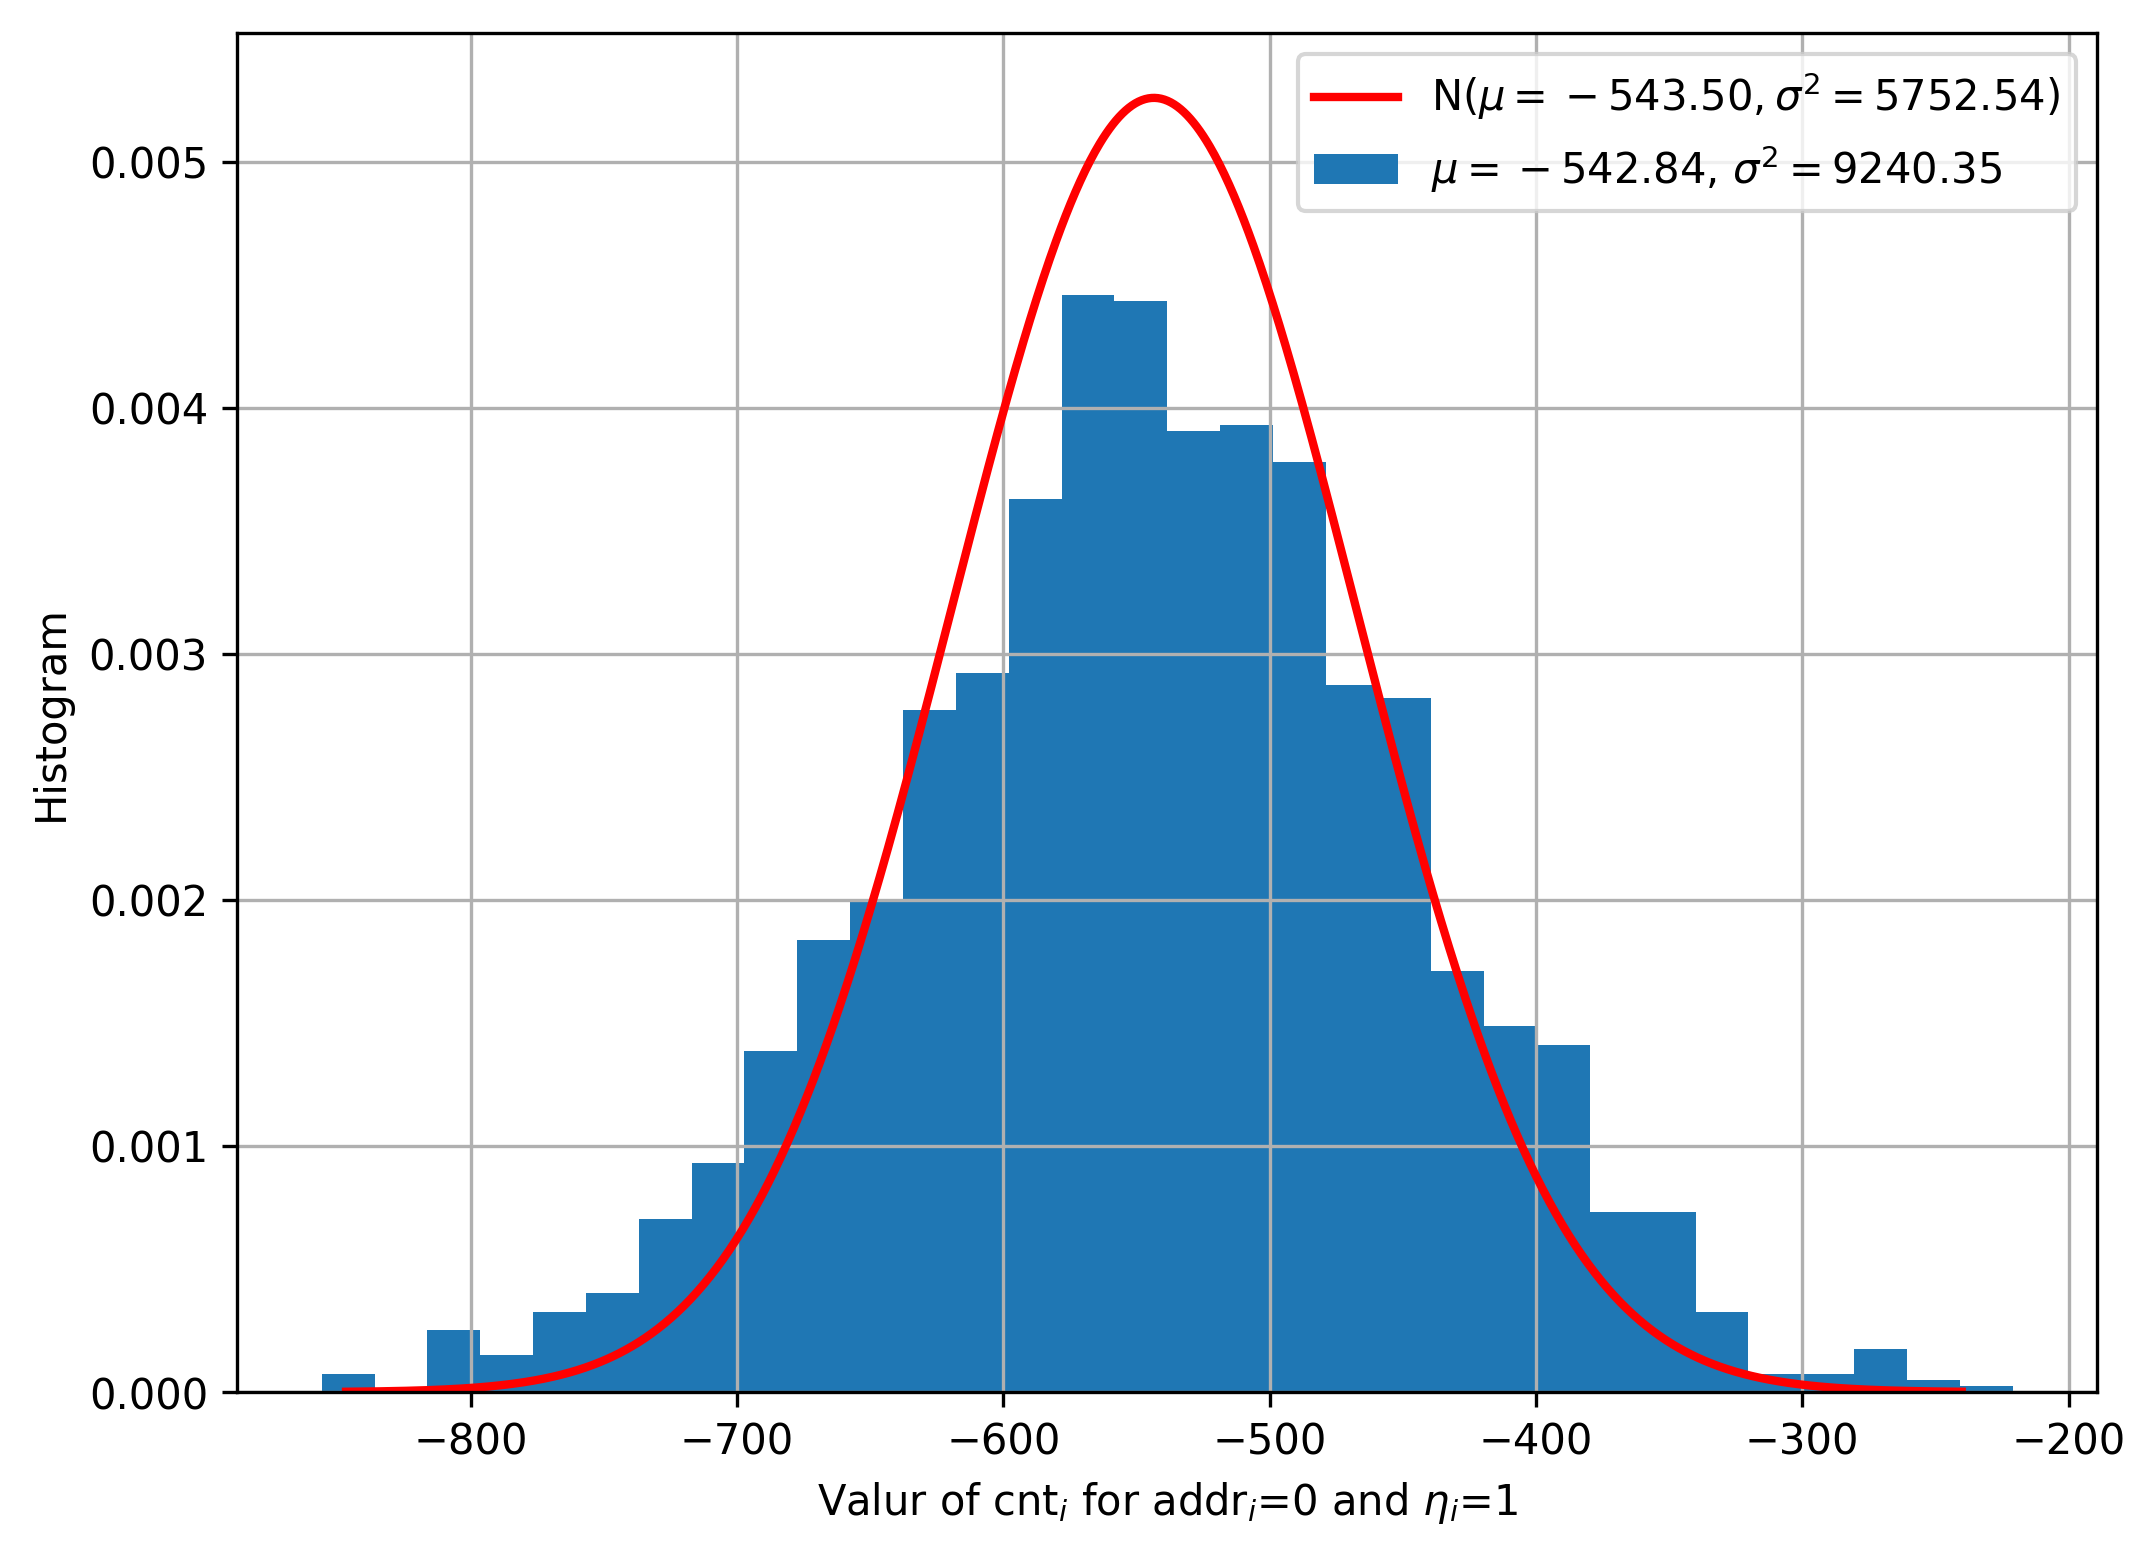
\includegraphics[width=0.5\textwidth]{./images02/autocorrelation/read-counters-eta1_addr0.png}}

  \caption{The histogram was obtained through simulation. The red curve is the theoretical normal distribution.}
  \label{fig:sdm-read-sums}
\end{figure}

Hence,

\begin{align}
\left[ \text{acc}_i|\eta_i=1 \right] &\sim \mathcal{N}(\mu = (2p-1)^2 \mu_\theta \mu_h, \sigma^2 = \sigma_\text{cnt}^2 \mu_h + 2 \mu_\text{cnt}^2 \sigma^2_h) \label{eqn:sdm-eta1} \\
\left[ \text{acc}_i|\eta_i=0 \right] &\sim \mathcal{N}(\mu = -(2p-1)^2 \mu_\theta \mu_h, \sigma^2 = \sigma_\text{cnt}^2 \mu_h + 2 \mu_\text{cnt}^2 \sigma^2_h) \label{eqn:sdm-eta0}
\end{align}

In our case, $\left[ \text{acc}_i|\eta_i=1 \right] \sim \mathcal{N}(\mu = 128.62, \sigma^2 = 12865.69)$, and $\left[ \text{acc}_i|\eta_i=0 \right] \sim \mathcal{N}(\mu = -128.62, \sigma^2 = 12865.69)$. See Figure \ref{fig:sdm-read} --- we can notice that the variance issue from Figure \ref{fig:sdm-read-sums} has propagated to these images.

\begin{figure}[h!]
  \centering
  \subfloat[Equation \ref{eqn:sdm-eta1}  ($\eta_k=1)$]{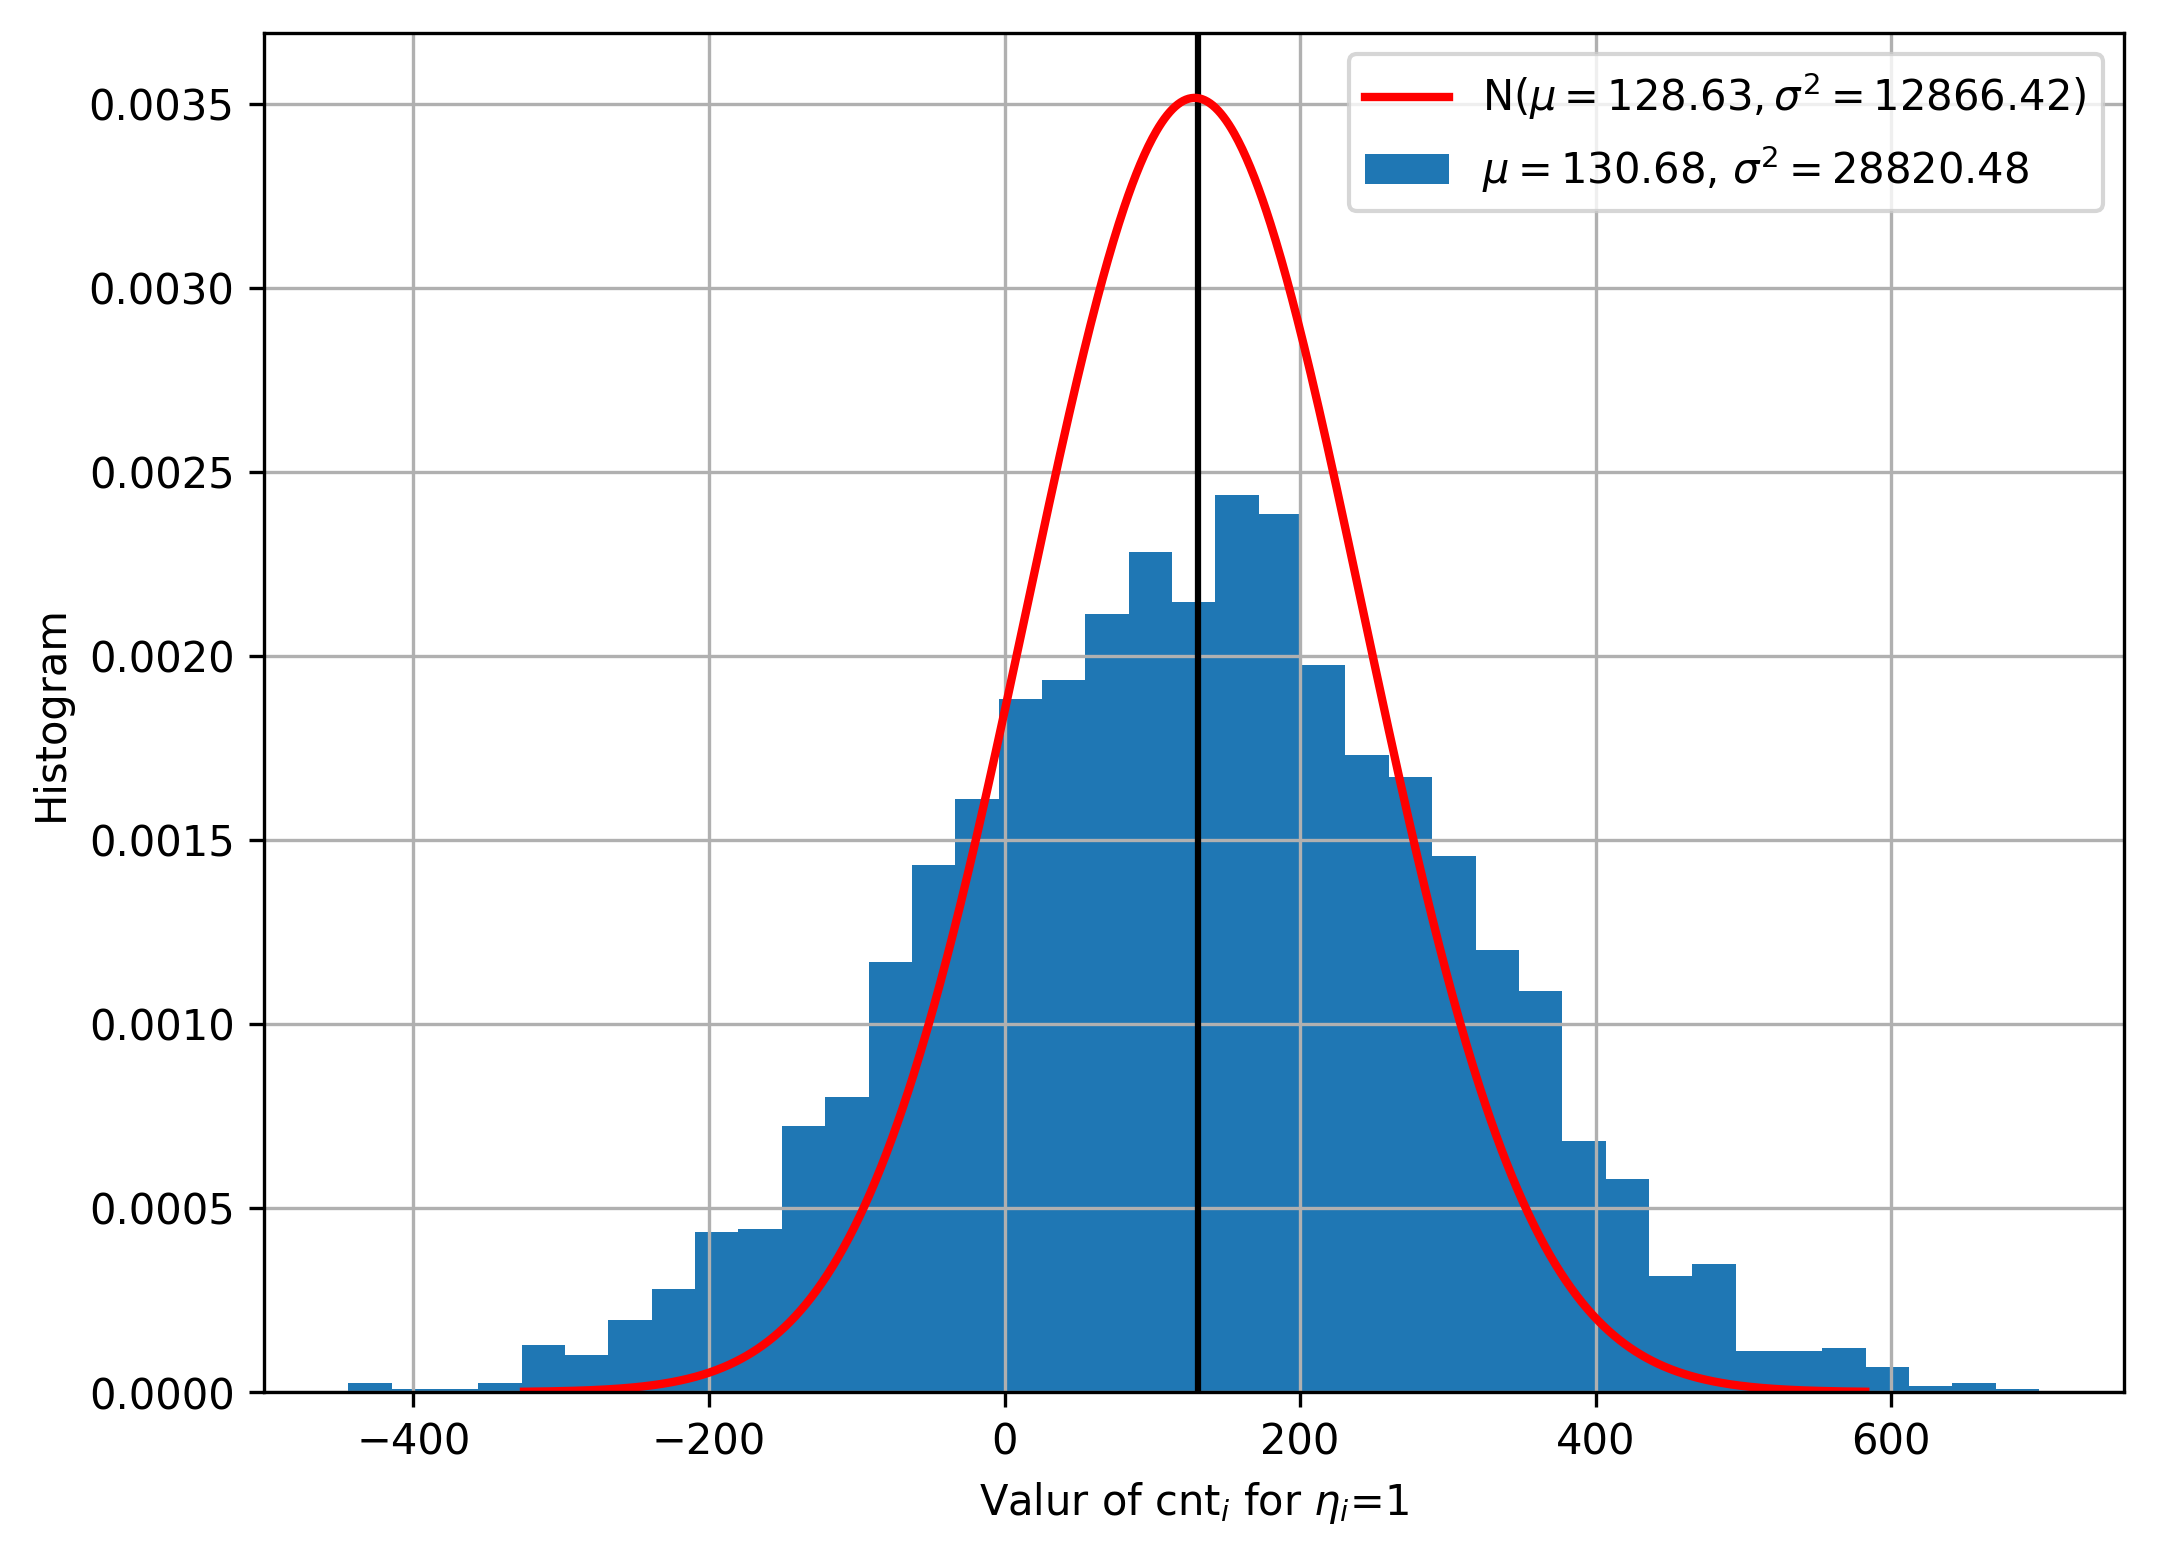
\includegraphics[width=0.5\textwidth]{./images02/autocorrelation/read-counters-eta1.png}}

  \subfloat[Equation \ref{eqn:sdm-eta0} ($\eta_k=0$)]{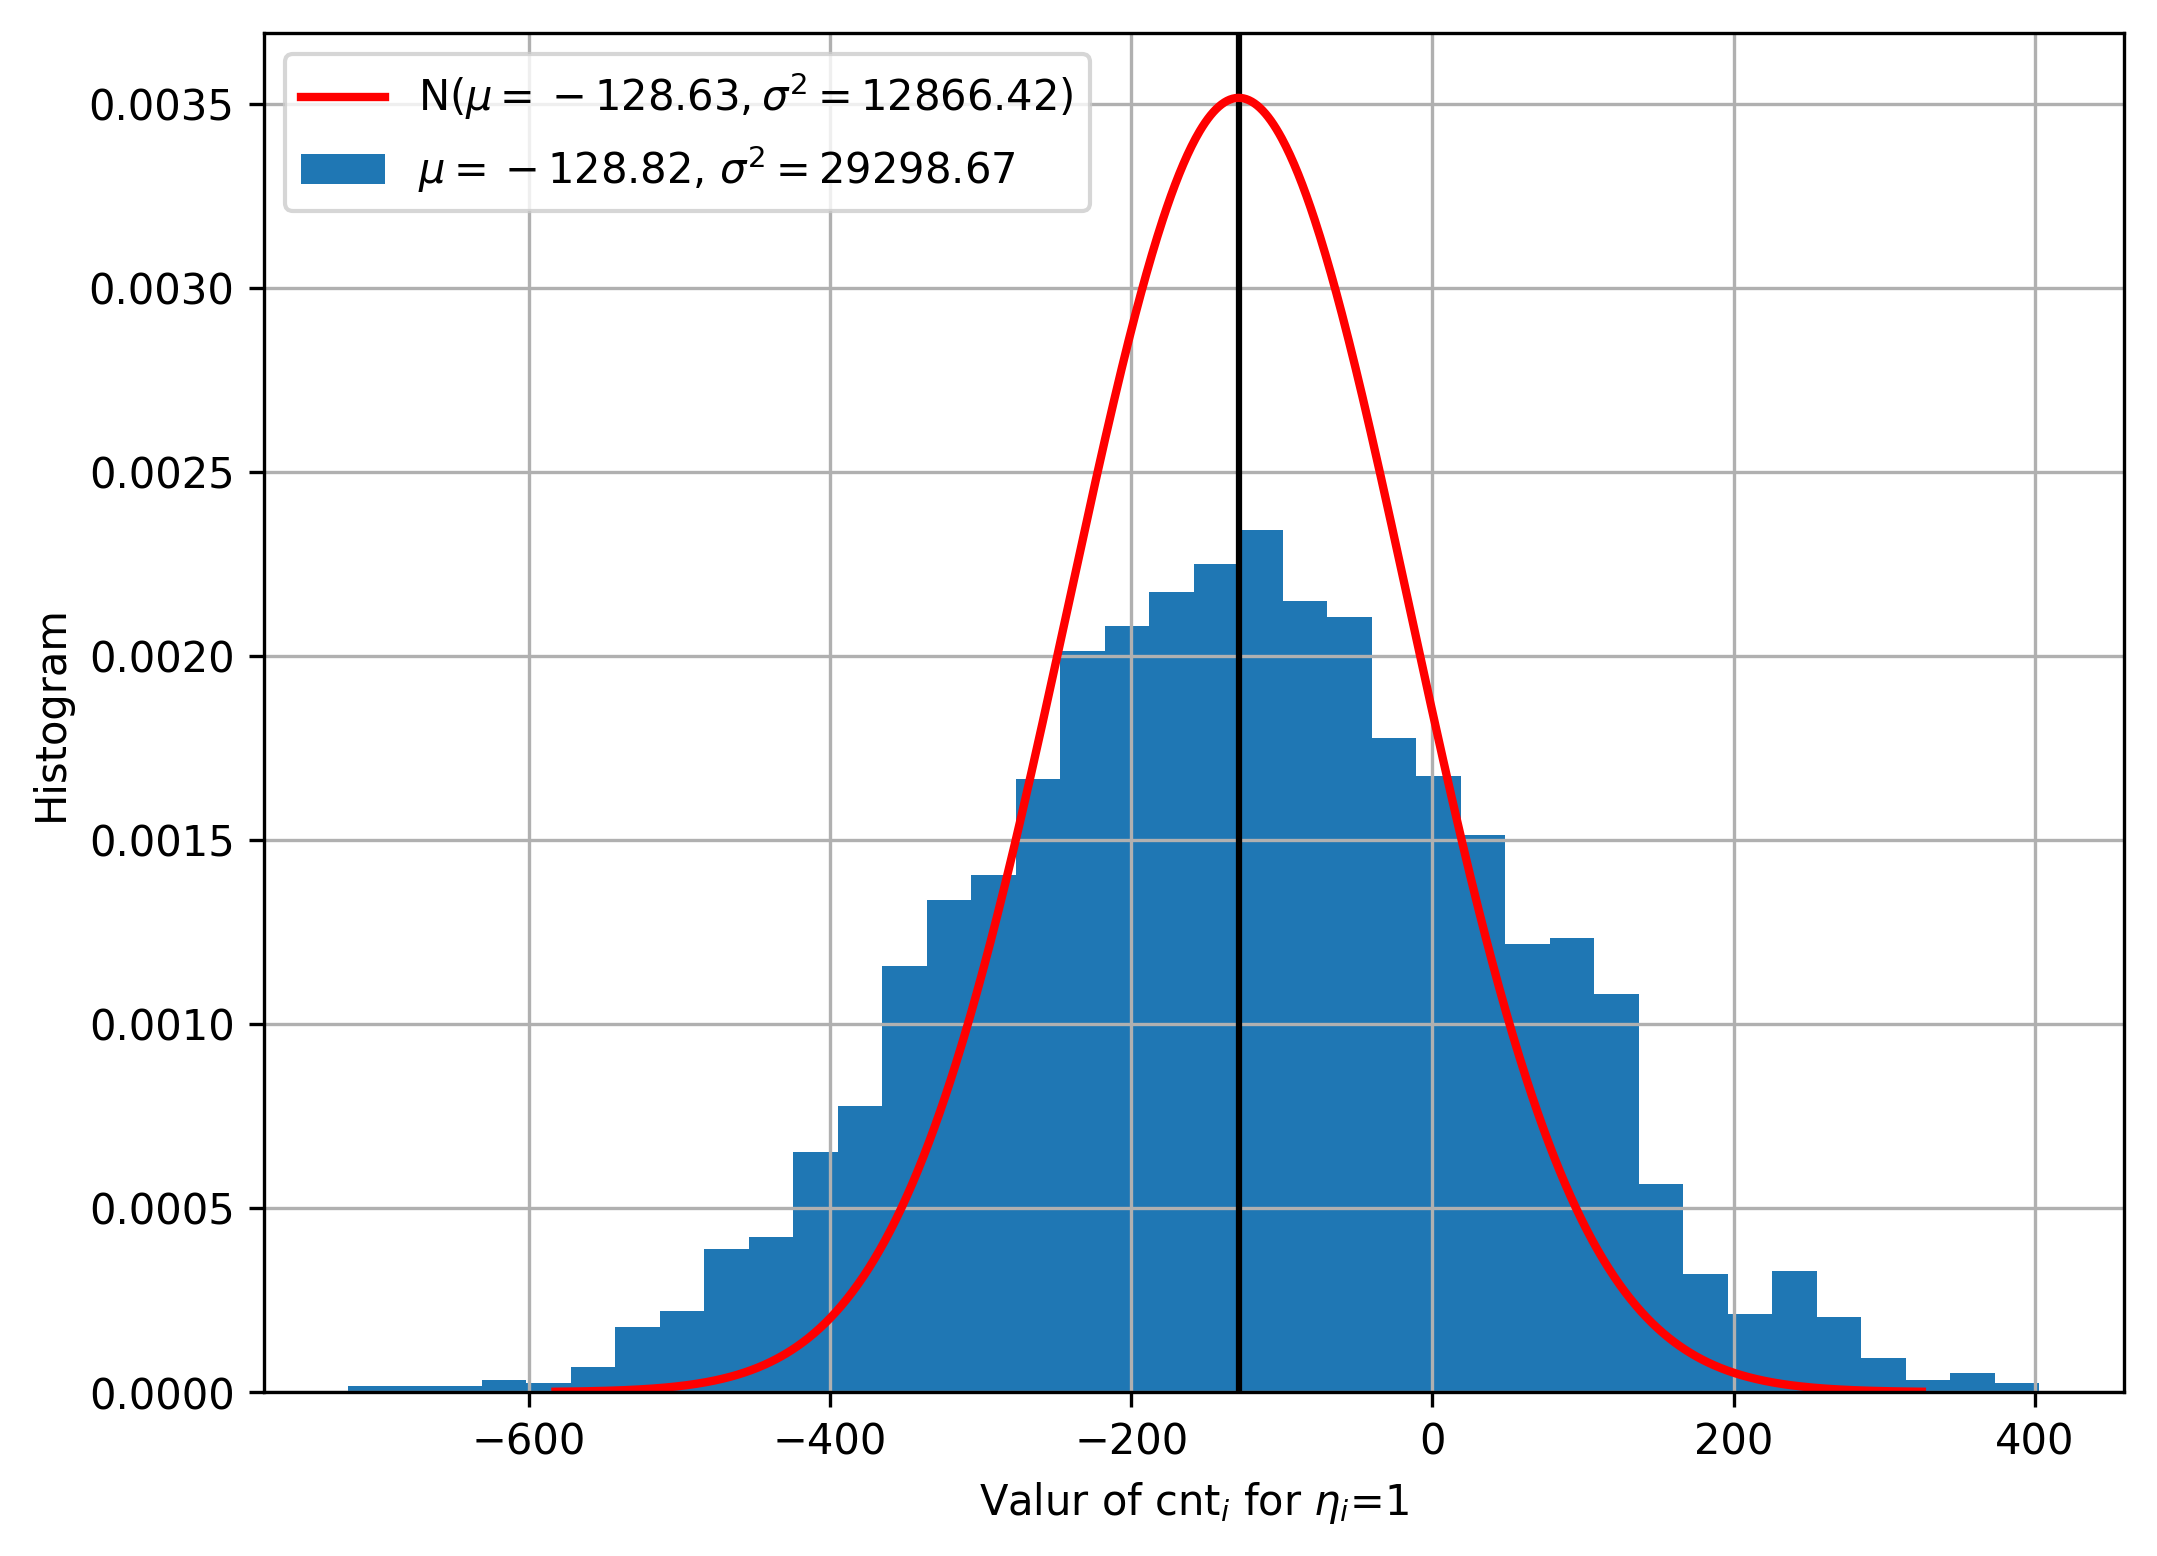
\includegraphics[width=0.5\textwidth]{./images02/autocorrelation/read-counters-eta0.png}}

  \caption{The histogram was obtained through simulation. The red curve is the theoretical normal distribution.}
  \label{fig:sdm-read}
\end{figure}


Finally,

\begin{align*}
P(wrong) = P(\text{acc}_i < 0 | \eta_i = 1) \cdot P(\eta_i = 1) {}& \\
+P(\text{acc}_i > 0 | \eta_i = 0) \cdot P(\eta_i = 0) \\
= \frac{\mathcal{N}_{\eta_i=1}.\text{cdf}(0)}{2} + \frac{1-\mathcal{N}_{\eta_i=0}.\text{cdf}(0)}{2} \\
= \frac{\mathcal{N}_{\eta_i=1}.\text{cdf}(0)}{2} + \frac{\mathcal{N}_{\eta_i=1}.\text{cdf}(0)}{2} \\
= \mathcal{N}_{\eta_i=1}.\text{cdf}(0)
\end{align*}





Using the empirical variance of $\sigma^2 = 27838.3029$, we calculate $P(wrong) = 0.220377$.

In order to check this probability, I have run a simulation reading from 1,000 random bitstrings (which have never been written into memory) and calculate the distance from the result of a single read. As the $P(wrong) = 0.22037$, I expected to get an average distance of 220.37 with a standard deviation of 13.10. See Figure \ref{fig:sdm-read-random-bs} for the comparison between the simulated and the theoretical outcomes.

Figure \ref{fig:sdm-single-read-dist} shows the new distance between $\eta_d$ and $\text{read}(\eta_d)$, where $\eta_d$ is $d$ bits away from $\eta$. As for $d \ge 520$ there is no intersection between $\eta$ and $\eta_d$, our models applies and explains the horizontal line around distance 220.

\begin{figure}[!htb]
  \centering
  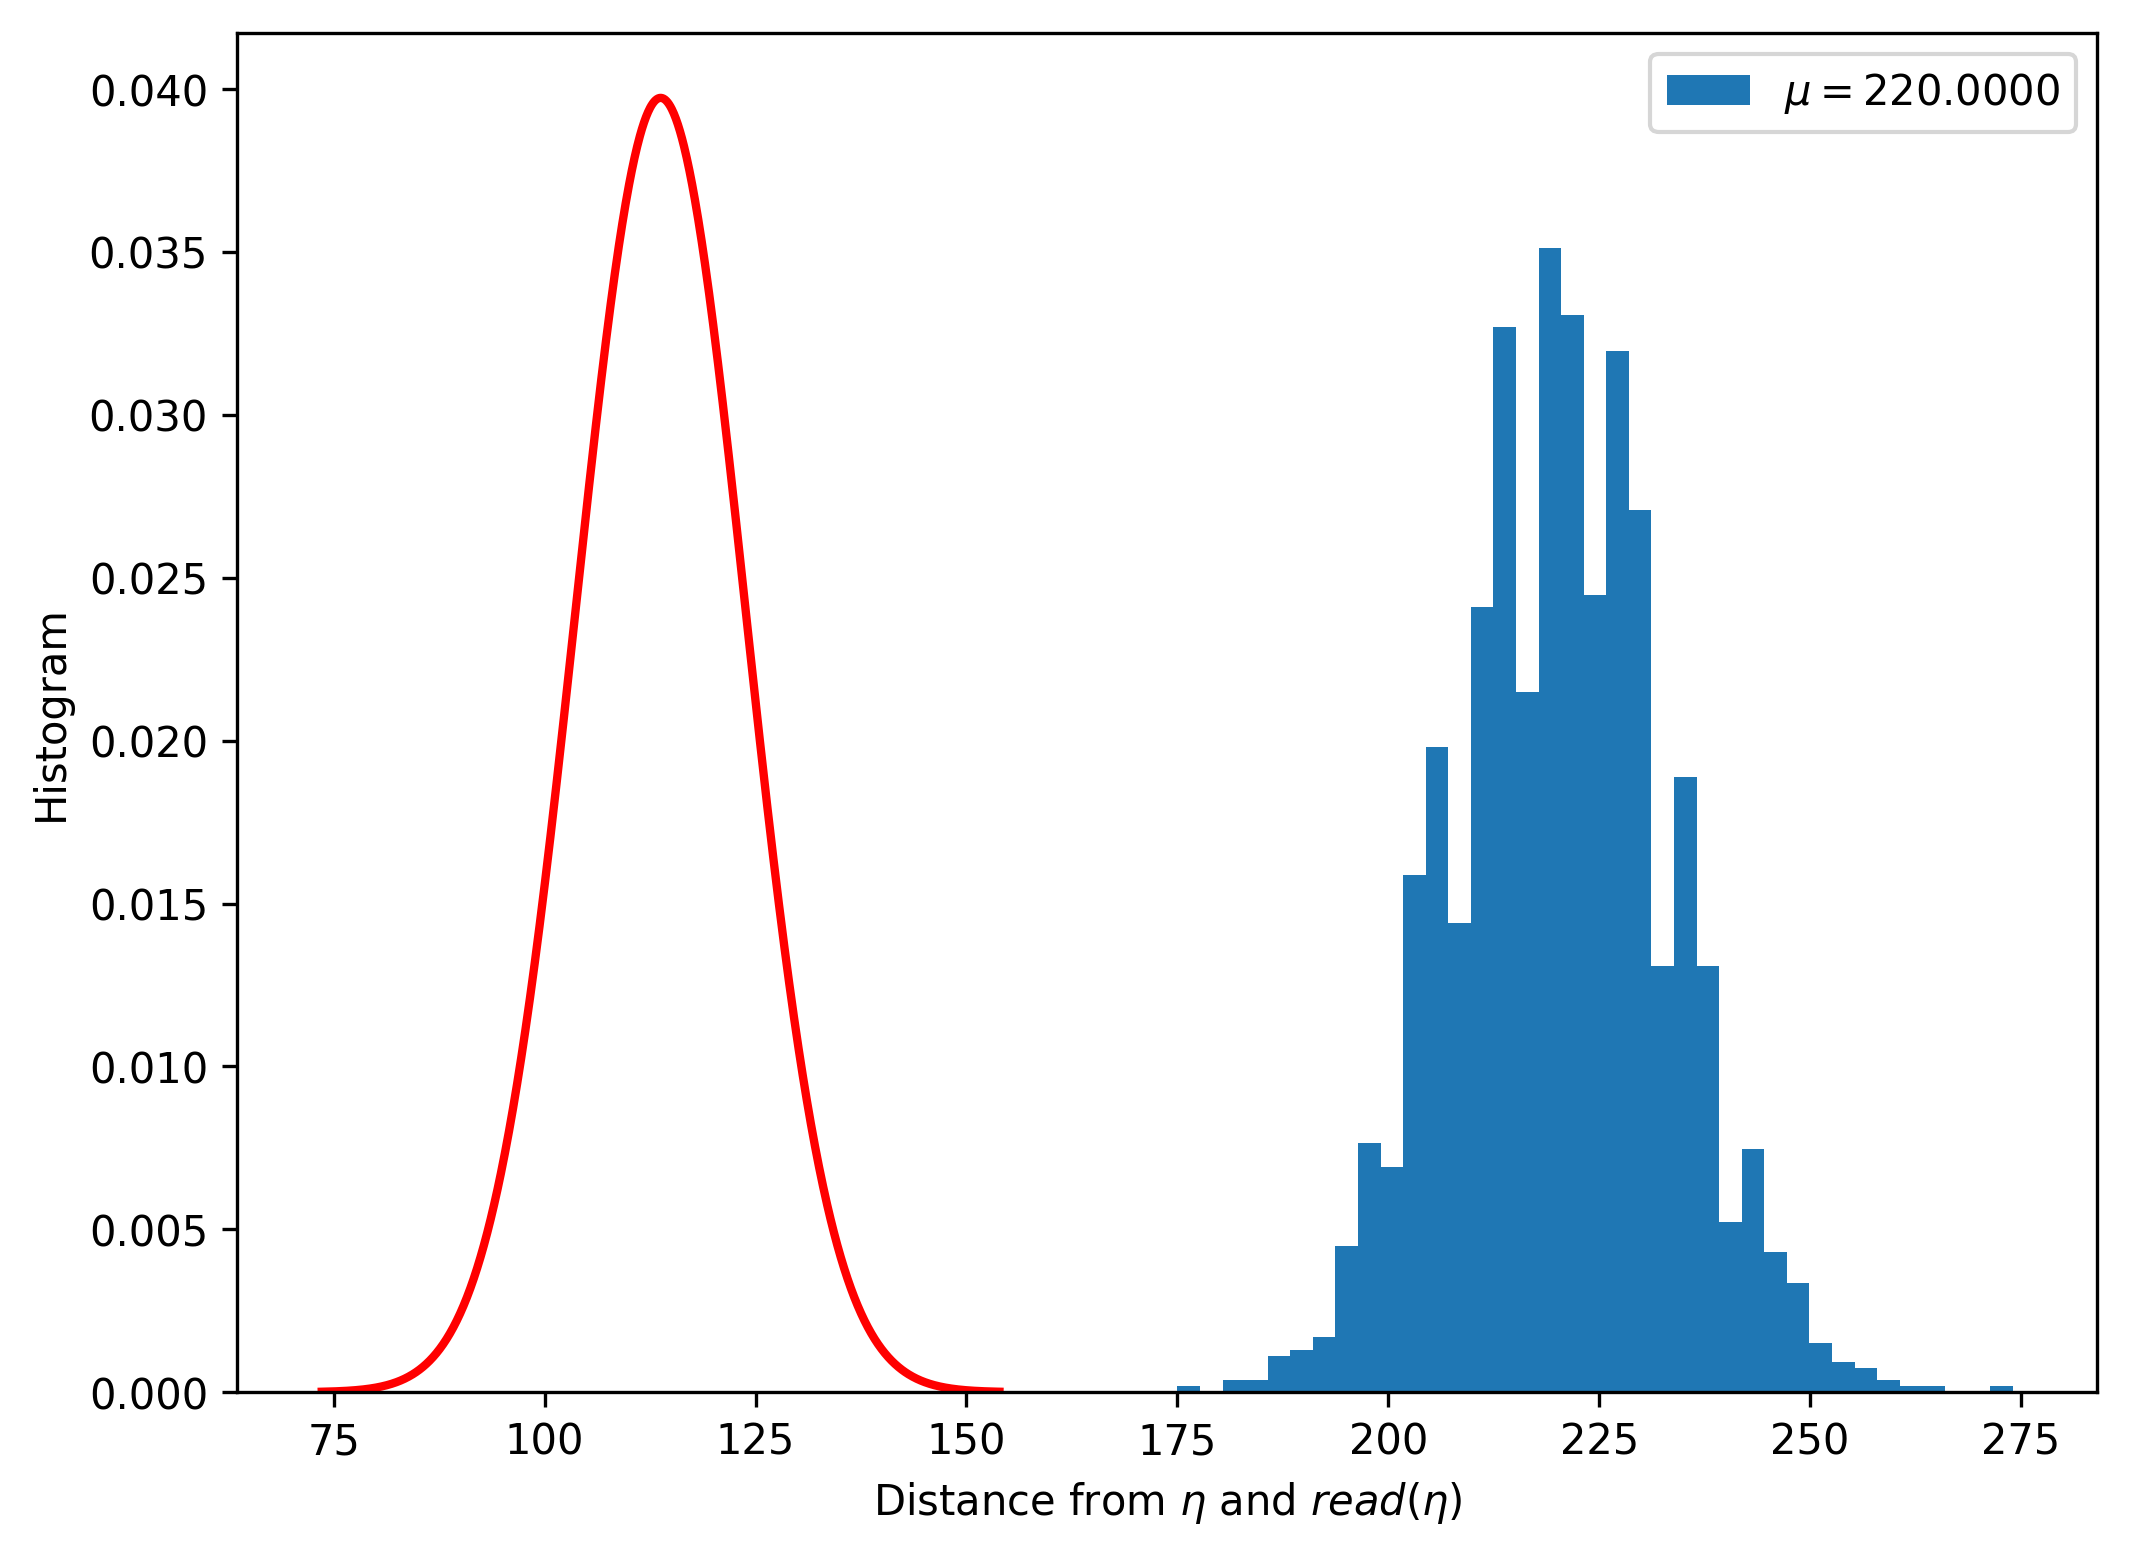
\includegraphics[width=0.5\textwidth]{./images02/autocorrelation/read-random-bs.png}

  \caption{The histogram was obtained through simulation. The red curve is the theoretical normal distribution.}
  \label{fig:sdm-read-random-bs}
\end{figure}

\begin{figure}[!htb]
  \centering
  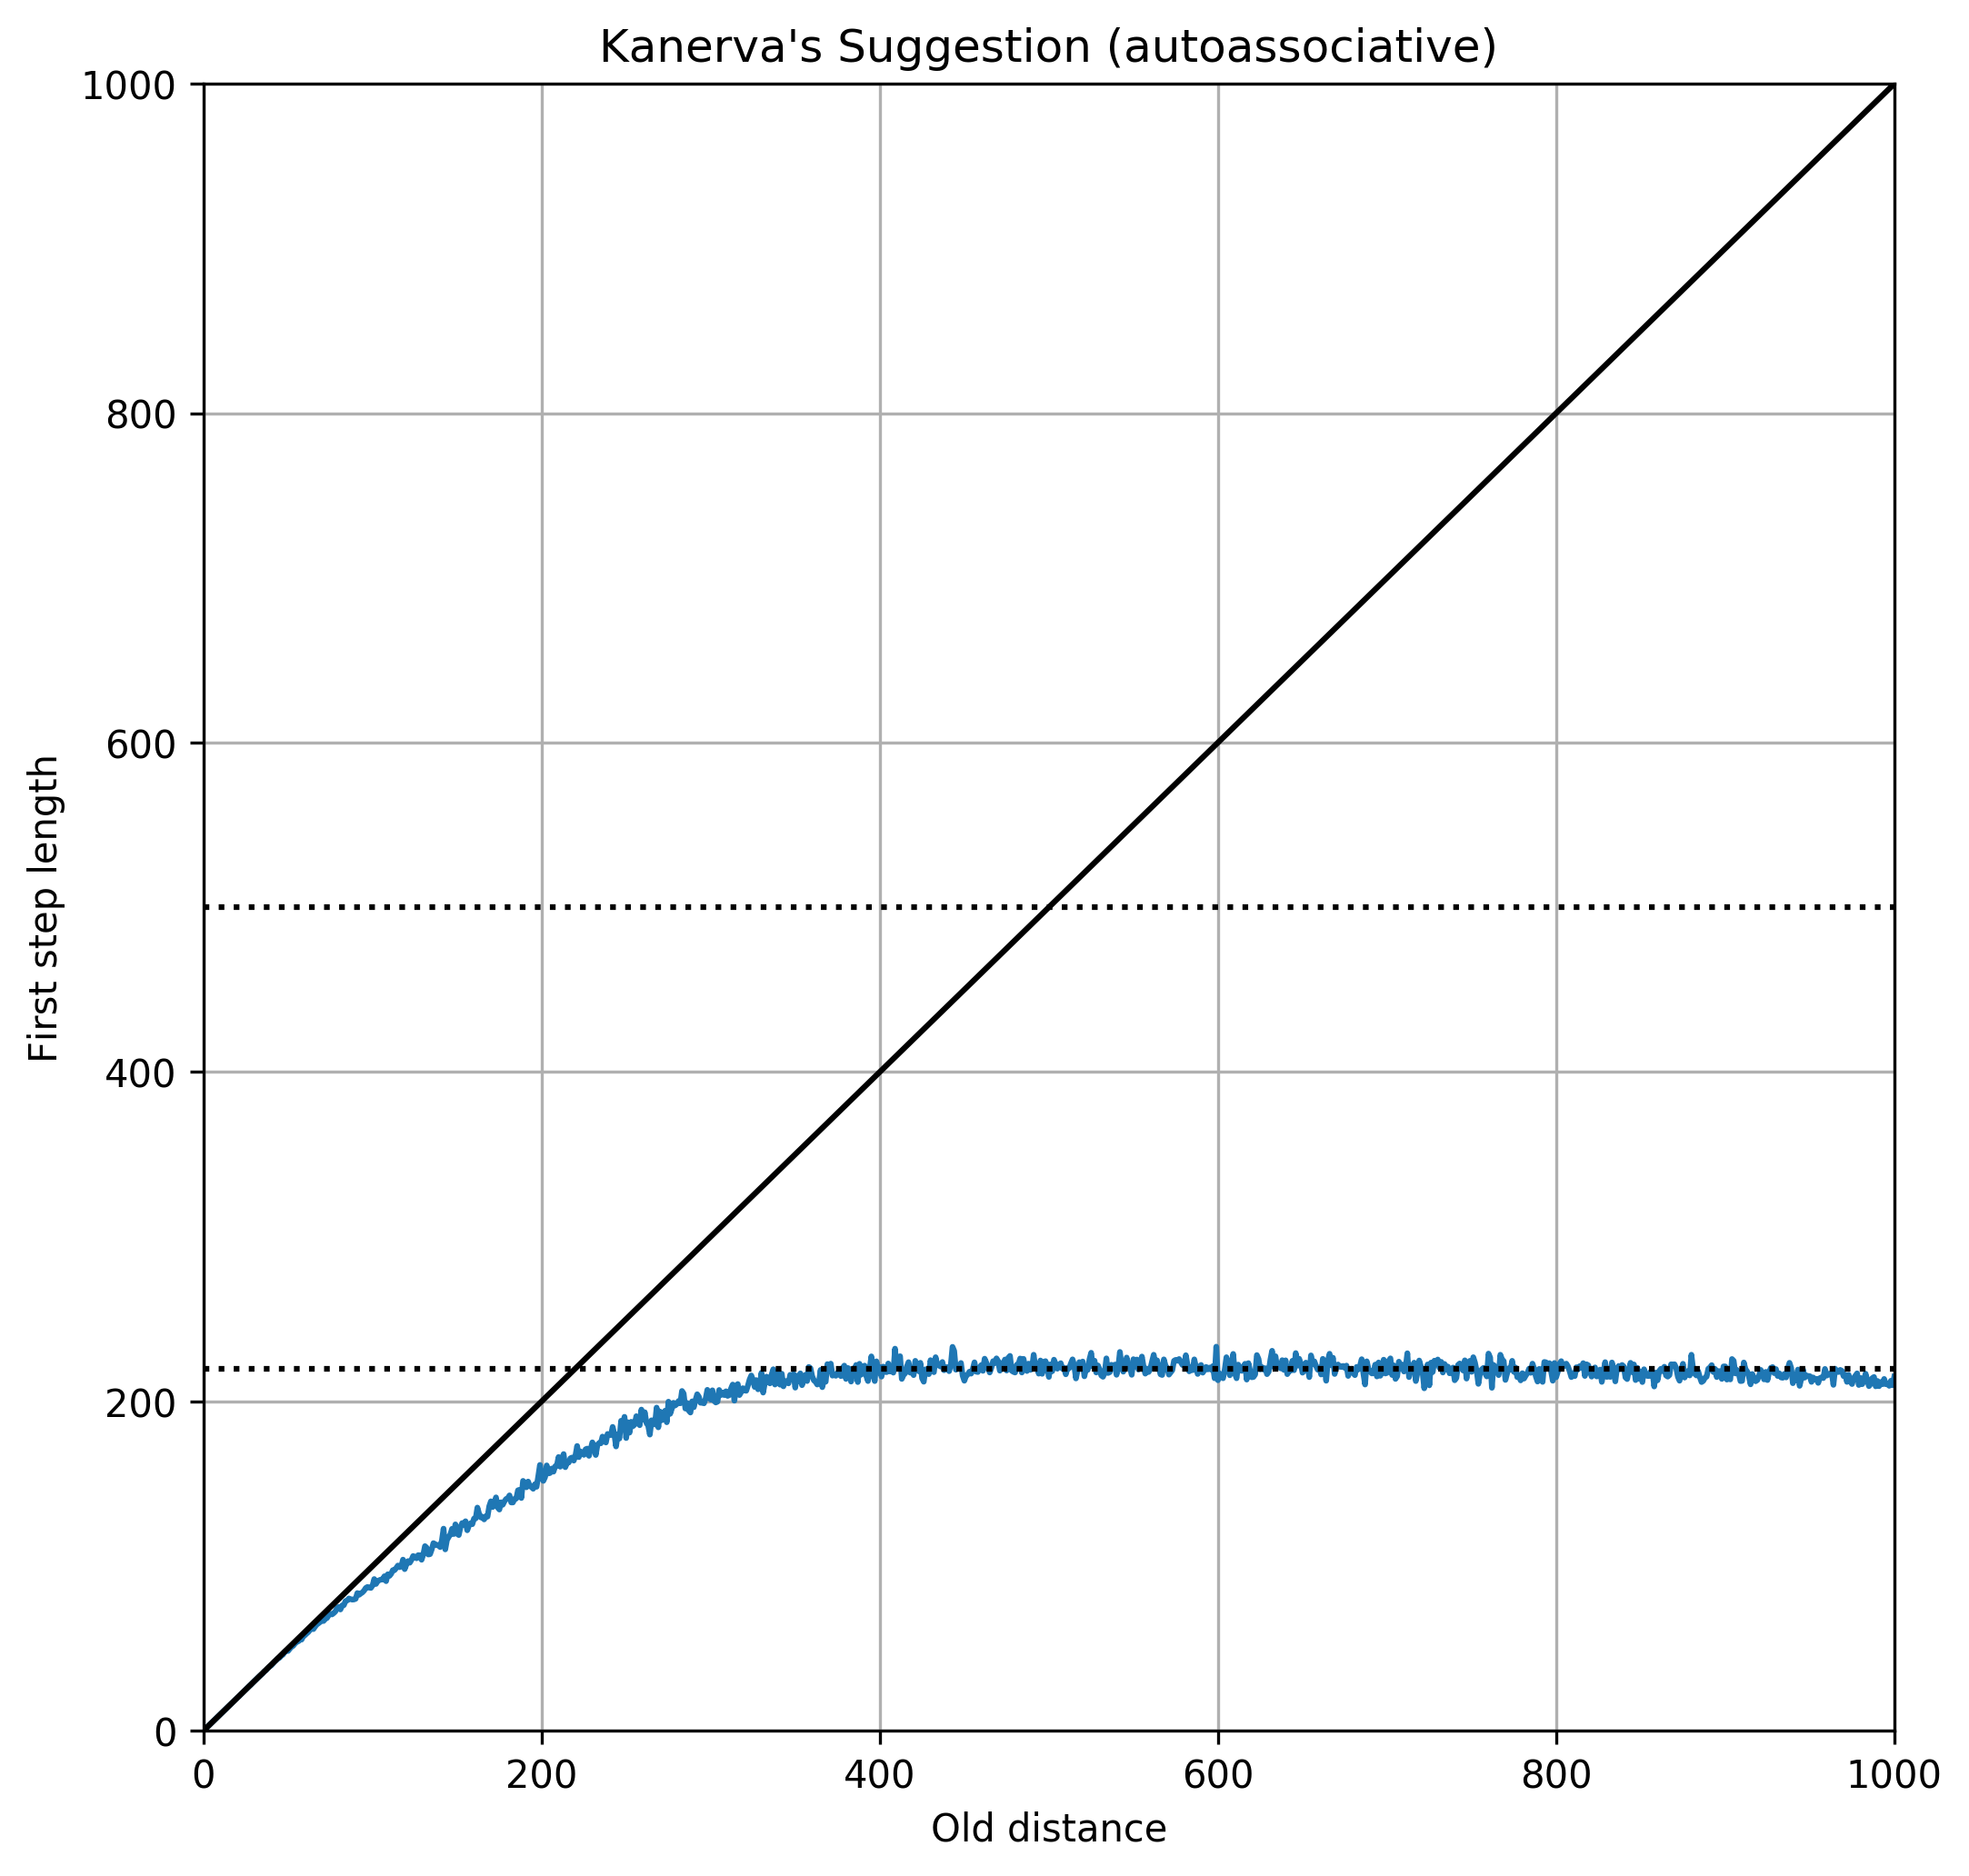
\includegraphics[width=0.5\textwidth]{./images02/autocorrelation/single-read-dist.png}

  \caption{New distance after a single read operation in a bitstring $\eta_d$, which is $d$ bits away from $\eta$. The new distance was calculated between $\eta_d$ and $\text{read}(\eta_d)$. Notice that when $d \ge 520$, the intersection between $\eta$ and $\eta_d$ is zero, which means there is only random bitstrings written into the activated hard locations. The distance 220 equals $1000 \cdot 0.220$ which is the probability find in Figure \ref{fig:sdm-read-random-bs}.}
  \label{fig:sdm-single-read-dist}
\end{figure}
